\documentclass[11pt]{article}
\usepackage{kotex}
\usepackage{fontspec}
\setmainfont{Times New Roman}
\setmainhangulfont[Ligatures=TeX]{AppleMyungjo}
\setsanshangulfont{Apple SD Gothic Neo}
\usepackage{amsmath,amssymb}
\usepackage{graphicx}
\usepackage{booktabs}
\usepackage{hyperref}
\usepackage{geometry}
\geometry{top=3cm,bottom=2.56cm,left=2.56cm,right=2.56cm}
\usepackage{setspace}
\setstretch{1.6}
\usepackage{titlesec}
\titleformat{\section}{\normalfont\large\bfseries}{\Roman{section}.}{0.5em}{}
\titleformat{\subsection}{\normalfont\normalsize\bfseries}{\arabic{section}.\arabic{subsection}}{0.5em}{}
\titleformat{\subsubsection}{\normalfont\normalsize\bfseries}{\arabic{section}.\arabic{subsection}.\arabic{subsubsection})}{0.5em}{}

\title{PolitiKAST: 정치 지식그래프 기반 다중 에이전트 유권자 궤적 시뮬레이션을 위한 한국 지방선거 검증 하네스}
\author{이성진(Seongjin Lee)\\BHSN}
\date{초안 -- \today}

\begin{document}

\maketitle

\begin{center}
\textbf{【국문초록】}
\end{center}
\noindent 본 연구는 대규모 언어 모형(Large Language Model, LLM), 한국형 합성 인구, 정치 지식그래프(Knowledge Graph, KG)를 결합하여 다직위(多職位) 지방선거에서 유권자 에이전트 시뮬레이션이 보류된 공식 여론조사 궤적을 재현할 수 있는지를 먼저 검증하는 validation-first 다중 에이전트 하네스를 제안한다. 각 유권자는 풍부한 사회·인구학적 속성과 기본 정치 성향을 갖춘 페르소나(persona)로 표현되며, 한국 공식 통계와 정렬된 합성 인구 자료로부터 구성된다. 언론 보도, 의혹 사건 수사, 법원 판결, 대변인 브리핑, 공표 여론조사 등 시간에 따라 변동하는 정보 환경은 선거 온톨로지와 담론 온톨로지에 기반한 사건 중심 정치 KG로 표현된다. 유권자 에이전트는 \texttt{LLMPool}/LiteLLM 기반의 얇은 커스텀 LLM 에이전트 계층으로 구현되며, KG의 관련 부분을 질의하고 시간에 따라 정당과 후보자에 대한 효용을 갱신한다. 본 연구는 (i) 언론·의혹 사건의 후보자 자질(valence) 효과, (ii) 공표 여론조사 노출에 대한 편승효과(bandwagon)와 약세효과(underdog), (iii) 정부 국정 운영 평가에 따른 이차 선거 동학, (iv) 동시 실시되는 다중 투표 간 상관된 선택, (v) 개인 수준 특성과 KG로 인코딩된 공유 정치 맥락의 명시적 분리를 함께 포착하는 수학적 모형을 도출한다. 본 틀은 선거 6개월 전부터 등록되는 공식 여론조사를 시간 순서대로 보정 구간과 보류 검증 구간으로 나누고, 각 검증 대상 여론조사의 조사·공표 시점 이전 정보만으로 모형 산출을 생성한 뒤 사후에 오차를 계산하는 rolling-origin 검증 파이프라인을 포함한다. 핵심적으로 공식 여론조사 결과는 유권자 prompt에 기본 제공되는 정보가 아니라 숨겨진 보정·검증 label이며, 보정된 설정을 동결한 뒤에는 후보 사퇴, 공천, 논란, 지지 선언 같은 사건열을 KG/시나리오에 주입해 반사실적 inference를 수행한다. 세 개의 사용 가능한 공식 사전 여론조사 target에 대해 clean no-cache 검증 gate를 두 단계로 실행했다. baseline $n{=}200$ clean run에서는 세 지역 모두 큰 오차와 함께 leader agreement에 실패했지만, KG Track A(인물·언론·사건·출처 narrative)와 Track B(연령 $\times$ 성별 CohortPrior 노드)를 KG에 박제하고 voter prompt에 코호트 사전정보 블록을 추가한 R6 full run에서는 평가 가능한 세 지역 모두에서 leader agreement를 회복하고, 평균 MAE가 $0.5066$에서 $0.1782$로 약 $2.84$배 개선되며, 대구시장은 지역별 시나리오 hardcode 없이도 MAE $0.0538$의 near-PASS에 도달했다. 서울시장은 $n{=}200$에서 코호트 사전정보 증폭으로 인한 share 과대편향 때문에 strict MAE gate를 통과하지 못해 §Limitations의 Track B caveat로 기록되었다. 광주와 대구 달서갑은 후보별 NESDC 검증 label이 여전히 부재하다. 따라서 본고는 2026년 지방선거의 검증된 예측을 주장하지 않고, 부분적으로 통과한 검증 gate를 보정 궤적으로 보고하며 반사실적 inference 프로토콜을 제시한다.

\vspace{0.5em}
\noindent\textbf{주제어:} 지방선거, 다중 에이전트 시뮬레이션, 대규모 언어 모형, 정치 지식그래프, 분할투표, 정당일체감

\section{서론}

선거 예측은 정치학과 정치 커뮤니케이션 분야의 오랜 핵심 과제이며, 구조적 거시 모형부터 여론조사 기반 현재예측(nowcast), 전문가 판단까지 다양한 접근이 존재해 왔다. 최근 LLM과 다중 에이전트 시스템의 발전은 새로운 연구 방향을 열었다. 즉, 정보를 소비하고 선호를 형성하며 가상으로 투표하는 수천에서 수백만 명의 프로그램적 에이전트로 구성된 인공 유권자 집단을 시뮬레이션하는 방향이다. 이 패러다임은 전통적 집계 모형보다 풍부한 반사실적 분석(\emph{이 의혹 사건이 없었다면 어떻게 되었을까?})과 투표 행동에 대한 보다 세밀한 설명을 제공할 가능성을 지닌다.

한국의 지방선거는 특히 매력적인 시험대다. 유권자는 종종 광역단체장, 기초단체장, 지방의회, 교육감 등 여러 직위에 대해 투표하며, 이러한 선택은 완전히 독립적이지도, 완전히 동일하지도 않다. 지방선거는 대통령 지지율과 ``정부 심판'' 같은 전국 차원 동학의 영향을 받지만, 동시에 지역 이슈, 후보자 valence, 선거운동 이벤트, 그리고 이들의 상호작용에서도 영향을 받는다. 따라서 지방선거와 보궐선거는 낮은 투표율과 항의 투표 유인을 갖는 이차 선거로 모형화한다~\cite{reif1980secondorder}. 또한 언론 보도, 부패 의혹, 검찰 수사, 법원 판결은 선거운동 기간 동안 후보자 평판을 변화시키고, 반복되는 여론조사는 유권자 기대를 측정하는 동시에 형성한다.

기존 접근법의 핵심 한계는 (i) 유권자를 동질적 집계로 다루어 미시 수준 이질성을 무시하거나, (ii) 각 유권자를 모든 관련 정보가 잠재 효용에 흡수된 고립 에이전트로 다루어 정치 맥락에 대한 명시적·공유 가능한 표현이 결여된다는 점이다. 이에 본 논문은 (a) 각 유권자를 인구통계와 정렬된 풍부한 페르소나로 표현하고, (b) 공유 정치 환경을 선거, 후보, 정당, 이슈, 사건, 여론조사를 포착하는 구조화된 지식그래프로 표현하는 이중 계층 아키텍처를 제안한다.

본 논문은 네 가지 기여를 한다.
\begin{itemize}
  \item 한국 지방선거를 동적 정보 환경 하의 다직위 선택 과제로 모형화하는 형식 문제를 정의하며, 합성 인구에서 추출된 페르소나와 정치 KG로 인코딩된 공유 맥락을 활용한다.
  \item 유권자 선호를 기본 성분, 언론·의혹 사건 valence 충격, 여론조사 피드백 효과, 정부 지지율 항으로 분해하고, 각 페르소나가 어떤 사건과 프레임에 노출되는지를 결정하는 KG 기반 정보 상태로 보강하는 효용 기반 모형을 도입한다.
  \item 대규모 한국 합성 페르소나 자료, 관계형 선거·여론조사 테이블, 사건 중심 KG, 시간 제한 검색 코퍼스를 통합하기 위한 구체적 데이터·저장소 아키텍처를 제시하며, 이질적 여론조사를 시간적으로 매끄러운 지지율 추정치로 집계하는 통합 여론조사 계층을 포함한다.
  \item \texttt{LLMPool}/LiteLLM 기반 다중 에이전트 구현과, 앞선 공식 여론조사로 보정하고 뒤따르는 보류 여론조사로 검증하되 해당 label을 유권자 prompt에는 기본 노출하지 않는 validation-first 실험 설계를 제시한다. 이후 동결된 설정으로 사건-KG intervention 기반 반사실적 inference를 수행하며, 선거 이후 지식 누출을 막는 시간적 정보 방화벽을 적용한다.
\end{itemize}

본 초안의 즉각적 목표는 zero-shot 선거 예측이나 여론조사 값을 prompt에 넣는 nowcast가 아니다. 목표는 KG 증강 페르소나 기반 선거 시뮬레이션을 숨겨진 공식 여론조사 label에 맞춰 보정·검증한 뒤, 설정을 동결하고 후보 사퇴·공천·논란·지지 선언 같은 사건 시나리오에 대한 반사실적 예측을 수행하는 프로토콜과 하네스 보고서다.

\begin{figure}[t]
\centering
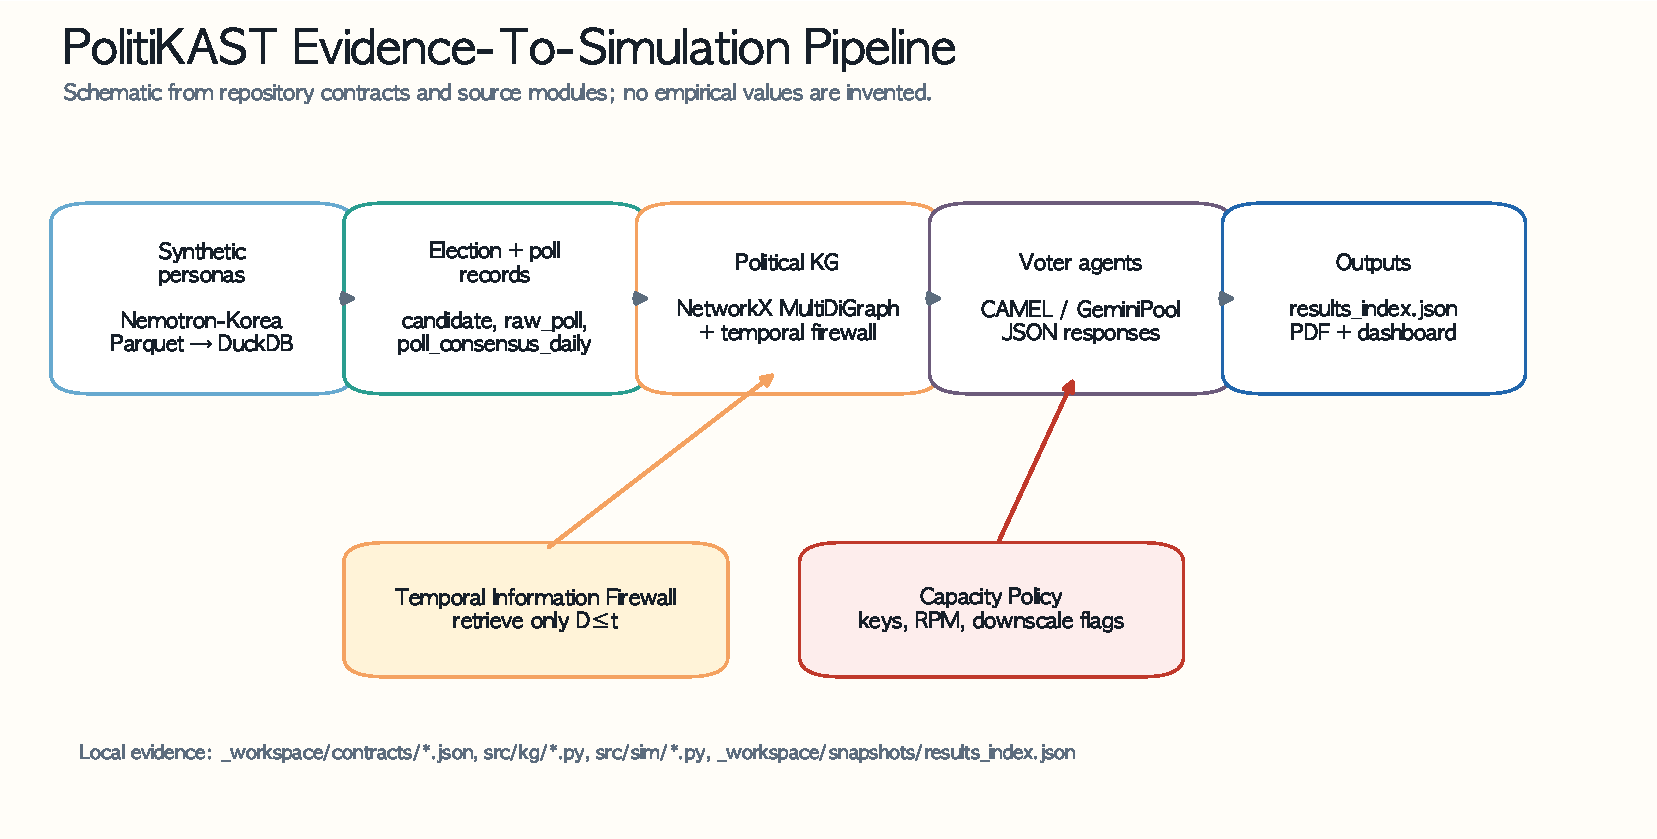
\includegraphics[width=\linewidth]{assets/fig_pipeline_architecture.pdf}
\caption{PolitiKAST 종단 간 파이프라인. 정적 페르소나 레코드와 관계형 선거 테이블은 유권자 및 경선 기반을 제공하고, 정치 KG, 시간적 정보 방화벽, LLMPool 기반 유권자 에이전트는 시간 제한 투표 결정과 후속 산출물을 생성한다.}
\label{fig:pipeline-architecture}
\end{figure}

\section{배경 및 관련 연구}

\subsection{언론, 의혹 사건, 정치 커뮤니케이션}

방대한 문헌은 정치 의혹 사건과 언론 보도가 선거 결과에 미치는 영향을 기록해 왔다. 실증 연구에 따르면 의혹 사건에 연루된 후보자는 일반적으로 득표율 감소와 재선 확률 하락을 겪으며, 그 효과는 의혹 사건 심각성, 언론 주목도, 전체 뉴스 환경에 따라 조절된다. 의혹 사건의 영향은 보통 초기에 집중되고 시간이 지남에 따라 감쇠하며, 그 결과는 당파성과 사전 신념에 따라 달라진다. 본 연구는 의혹 사건 효과를 확률적 penalty로 다루는데, meta-analysis가 득표 손실은 찾지만 투표율 효과는 모호하다고 보기 때문이다~\cite{solaz2018scandalmeta}.

의혹 사건을 넘어, 정당과 정부의 전략적 커뮤니케이션---대변인 브리핑과 기자회견---은 이슈를 프레이밍하고 인지된 후보자 valence를 형성한다. 언론 혼잡, 이슈 경쟁, 의혹 사건 가능성 사이의 상호작용은 특정 사건이 유권자에게 반향을 일으키는지, 경쟁 보도에 묻히는지를 좌우한다.

\subsection{여론조사와 편승효과·약세효과}

여론조사는 선거 동학에서 이중 역할을 한다. 한편으로 여론조사는 표본 오차와 방법별 편향을 안고 현재 지지율을 측정한다. 다른 한편으로 공표된 여론조사 결과는 편승효과(인지된 승자에 합류) 또는 약세효과(뒤처진 후보에 결집) 같은 행동 반응을 유발할 수 있다. 현장 및 설문 실험은 여론조사 정보가 결정이 늦거나 약하게 결속된 유권자에게 영향을 줄 수 있음을 보여주지만, 효과 크기와 방향은 맥락에 따라 다양하다. 기본 prior는 survey experiment가 일관된 편승효과와 약세효과 부재를 보고한다는 점을 반영해 약세효과보다 편승효과를 더 크게 둔다~\cite{hansen2016polls}.

따라서 여론조사와 최종 선거 결과의 관계는 내생적이다. 여론조사는 유권자 선호를 반영하면서도 정보 환경과 유권자 기대에 다시 피드백한다. 여론조사와 선거를 함께 예측하려는 시뮬레이션은 이러한 피드백 루프를 명시적으로 모형화해야 한다.

\subsection{이차 선거(second-order election)와 정부 심판}

``이차 선거(second-order election)'' 이론은 지방·초국가 선거(예: 지방, 광역, 유럽의회)가 종종 지역 이슈를 직접 결정하기보다는 중앙 정부를 보상하거나 처벌하는 데 사용된다고 본다. 실증적으로 여당은 중간선거나 저주목 선거에서 더 부진한 경향이 있으며, 정부 지지율은 지방선거 결과의 강한 예측 변수다. 한국 맥락에서 혼합형 선거제도와 지방선거는 제도 설계, 전략 투표, 정부 평가가 상호작용하는 풍부한 환경을 제공한다. 한국 유권자는 비례대표와 지역구 투표가 공존하는 상황에서도 전략투표를 보일 수 있다~\cite{choi2006strategic}.

\subsection{한국 선거에서의 분할투표}

분할투표---같은 선거에서 직위별로 다른 정당에 표를 던지는 행위---는 혼합형·다층 선거제도에서 널리 관찰된다. 한국 연구는 분할투표 행태가 약한 당파성, 특정 사회·인구학적 프로필, 정부 성과 평가와 연관됨을 보여준다. 유권자는 지역구 선거에서는 한 정당을, 비례대표나 지방 경선에서는 다른 정당을 지지할 수 있으며, 이는 전국 및 지역 차원 고려를 함께 반영한다. 2004년 한국 유권자의 약 20\%가 지역구와 정당명부 투표를 분할했다는 근거에 따라 분할투표 전이 prior를 둔다~\cite{splitticket_korea}.

이러한 발견은 모든 투표 직위가 공통 잠재 요인(이념, 정당일체감, 정부 지지)을 공유하면서도 직위별 성분과 특이 변동을 함께 포함하는 모형을 동기 부여한다. 직위 간 상관 구조는 일관투표와 분할투표의 현실적 패턴을 포착하는 데 필수적이다.

\subsection{에이전트 기반 선거 예측}

에이전트 기반 모형(ABM)은 유권자를 선호와 사회적 연결을 가진 개별 에이전트로 표현하며 선거운동 동학과 투표율을 시간에 따라 시뮬레이션한다. 최근 연구는 ABM이 에이전트 수준 모수를 여론조사와 과거 결과에 보정함으로써 실제 선거를 성공적으로 예측할 수 있음을 보여준다. 집계 예측은 대체로 개별 유권자를 직접 포함하지 않기 때문에 에이전트 기반 선거 예측이 유용하다~\cite{gergaud2022abmelections}. 이러한 모형은 계산적 제약 때문에 비교적 단순한 행동 규칙과 저차원 유권자 속성에 의존하는 경우가 많다.

\subsection{LLM 기반 투표와 다중 에이전트 프레임워크}

LLM Voting에 관한 최근 연구는 LLM 에이전트가 투표 시나리오에서 어떻게 선택을 하는지, 집단적 결정이 인간 선호와 어떻게 비교되는지, 프롬프트와 의사결정 규칙이 결과에 어떻게 영향을 미치는지를 탐구한다. 이러한 연구는 전체 유권자 집단을 직접 시뮬레이션하지는 않지만, 언어 모형이 다양한 정보·프레임 조건 하에서 구조화된 의사결정을 근사할 수 있음을 보여주며, 동시에 투표지 순서, 페르소나 명세, temperature가 LLM 집단 결과를 이동시킬 수 있음을 시사한다~\cite{yang2024llmvoting}. ElectionSim은 미국 대선 시나리오에서 백만 단위 LLM 유권자 시뮬레이션을 보였고~\cite{liu2024electionsim}, PolitiKAST는 KG 기반 시간 맥락을 가진 한국 지방선거에 초점을 둔다.

엔지니어링 측면에서 CAMEL과 같은 다중 에이전트 라이브러리는 대규모 상호작용 LLM 에이전트 집단을 생성·조율·확장하는 추상화를 제공한다. CAMEL은 에이전트 역할, 사회, 통신 패턴 정의 원시 도구뿐 아니라 외부 데이터 및 도구 통합 도구도 제공한다. 이 프레임워크는 미시 수준 결정에 LLM을 활용하면서도 거시 구조와 모수에 대한 명시적 통제를 유지하는 선거 시뮬레이션 엔진의 자연스러운 토대다.

\subsection{한국형 에이전트를 위한 합성 페르소나}

공식 통계와 행정 데이터로 구축된 합성 인구 자료은 식별 가능한 개인 데이터에 의존하지 않고 정책·선거 시나리오의 미시 시뮬레이션을 가능하게 한다. 한국 맥락에서는 최근 국가 통계 및 관련 자료로부터 도출된 인구통계 분포(지역, 연령, 성별, 직업, 소득, 가구 유형)와 정렬된 수백만 합성 개인 페르소나 자료이 공개되었다. 이러한 자료은 표 속성과 개인별 다중 페르소나 서사를 모두 노출하며, LLM 기반 선거 시뮬레이션의 기본 에이전트 풀로 적합하다~\cite{bhattacharjee2024nemotron}.

\subsection{정치 온톨로지와 지식그래프}

선거·정치 온톨로지는 선거, 경선, 정당, 후보, 선거구, 결과를 모형화하기 위한 구조화된 어휘를 제공한다. KG schema는 election, candidacy, electorate, constituency, party, result 같은 선거 개념을 재사용하며 공공 선거 온톨로지 관행과 정렬된다~\cite{ukparl_election_ontology}. 뉴스로부터 구축된 사건 중심 지식그래프는 정치 사건, 행위자, 이슈를 표현하여 복잡한 질의와 시각 분석을 지원해 왔다.

최근에는 연설, 토론, 언론 서사를 이슈, 프레임, 행위자에 연결된 구조화된 개체로 표현하는 정치 담론 온톨로지·지식그래프가 제안되었다. 뉴스룸 지향 KG 플랫폼은 개체·사건 연결을 통해 저널리즘 워크플로우를 지원하는 방법을 보여준다. 이러한 연구는 본 프레임워크의 정치 KG 설계에 영감을 준다. 즉, 선거와 제도가 구조적 골격을 제공하고, 사건과 서사가 시간 차원을 채운다.

\section{데이터 및 저장소 아키텍처}

\subsection{페르소나 계층: 관계형 코어 + 서사 텍스트}

\paragraph{합성 인구.}
본 연구는 NVIDIA가 공개한 Nemotron-Personas-Korea~\cite{bhattacharjee2024nemotron}(CC BY 4.0)를 사용한다. 이 자료는 한국의 인구학적·지리적 분포에 기반한 \textbf{1{,}004{,}752개 레코드와 약 700만 개 페르소나 서술}을 제공한다. 각 레코드는 26개 필드를 노출하며, (i) \texttt{persona}, \texttt{professional\_persona}, \texttt{sports\_persona}, \texttt{arts\_persona}, \texttt{travel\_persona}, \texttt{culinary\_persona}, \texttt{family\_persona} 등 일곱 개 서사 필드, (ii) \texttt{cultural\_background}, \texttt{skills\_and\_expertise}, \texttt{hobbies\_and\_interests}, \texttt{career\_goals\_and\_ambitions} 등 자유형 속성 필드, (iii) 17개 시도와 252개 행정구역을 포괄하는 인구·지리 필드 및 UUID 기본 키로 구성된다. 자료는 만 19세 이상 성인만 포함하며, 세부 직업과 생애 경로 표본 추출에는 여러 인구학 요인 사이의 조건부 독립을 가정하는 확률적 그래프 모형(PGM)이 사용된다. 이 한계는 제~\ref{sec:limitations}절에서 논의한다.

\begin{figure}[t]
\centering
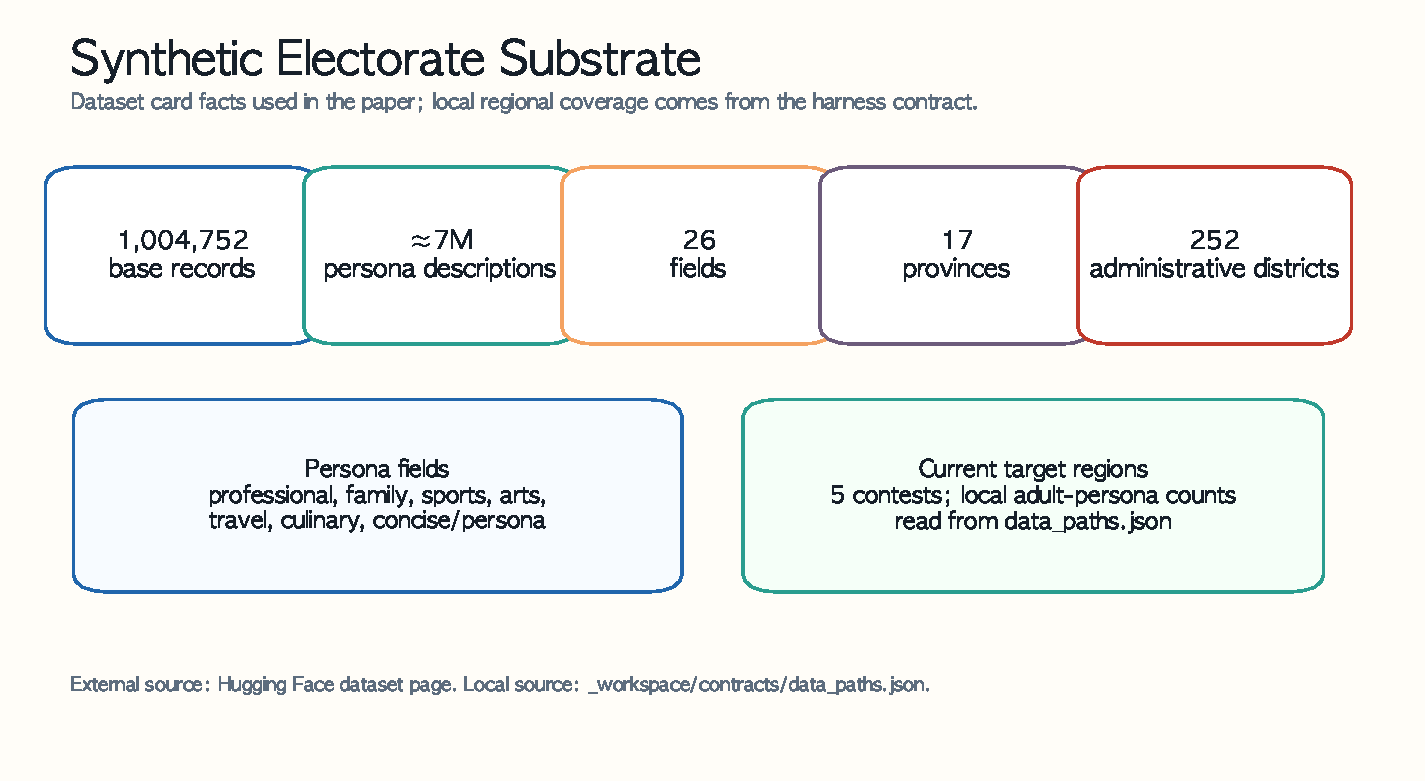
\includegraphics[width=0.92\linewidth]{assets/fig_persona_data_card.pdf}
\caption{Nemotron-Personas-Korea 페르소나 계층 데이터 카드. 카드는 시뮬레이터 설계에 쓰이는 공개 자료 속성만 기록하며, 한국 투표연령 시뮬레이션에서 중요한 성인 전용 커버리지 한계를 강조한다.}
\label{fig:persona-data-card}
\end{figure}

자료는 로컬 Parquet 파일 9개 샤드에서 읽어 DuckDB로 인제션된다. 각 레코드는 표 속성과 다중 페르소나 서사를 모두 제공한다. 효율적 표본 추출, 결합, 집계를 지원하기 위해 페르소나 데이터를 두 관계형 테이블에 저장한다.

\begin{itemize}
  \item \textbf{persona\_core}: 페르소나당 한 행으로 인구통계 및 지리 속성 컬럼을 포함한다.
  \begin{itemize}
    \item \texttt{uuid} (UUID 기본 키), \texttt{province}, \texttt{district}, \texttt{sex}, \texttt{age}, \texttt{marital\_status}, \texttt{military\_status}, \texttt{family\_type}, \texttt{housing\_type}, \texttt{education\_level}, \texttt{bachelors\_field}, \texttt{occupation}.
  \end{itemize}
  \item \textbf{persona\_text}: 페르소나당 한 행으로 장문 서사 필드를 포함한다.
  \begin{itemize}
    \item \texttt{persona}, \texttt{professional\_persona}, \texttt{family\_persona}, \texttt{travel\_persona}, \texttt{culinary\_persona}, \texttt{arts\_persona}, \texttt{sports\_persona}, \texttt{cultural\_background}, \texttt{skills\_and\_expertise}, \texttt{hobbies\_and\_interests}, \texttt{career\_goals\_and\_ambitions}.
  \end{itemize}
\end{itemize}

이 설계는 기반 자료의 표 구조를 반영하며 계층적 표본 추출과 집계를 위한 지역·인구통계 인덱싱을 가능하게 한다. 서사 필드는 필요 시 유권자 에이전트 프롬프트에 주입되지만 대부분의 DB 질의에서는 필요하지 않다. 현재 하네스는 이 페르소나 원천을 성인 전용 자료로 취급하며, 한국 투표연령에 만 18세 유권자가 포함된다는 점을 명시적 한계로 기록한다.

\subsection{선거 및 결과 테이블}

선거 구조와 결과는 다음과 같은 관계형 스키마에 저장된다.

\begin{itemize}
  \item \textbf{election}: 선거별 메타데이터(유형, 연도, 범위).
  \item \textbf{contest}: 투표 직위(예: 광역단체장, 기초단체장)당 한 행으로 선거, 선거구, 직위 정보.
  \item \textbf{party}: 정당 식별자와 속성.
  \item \textbf{candidate}: 후보자 식별자, 정당 연결, 현직 여부, 이력.
  \item \textbf{result}: 선거구·후보·경선별 실제 득표 및 득표율.
\end{itemize}

이 테이블은 KG 계층이 참조하는 구조적 골격을 형성한다.

\subsection{여론조사 데이터: 원시 아카이브와 통합 계층}

여론조사는 두 계층으로 저장된다.

\paragraph{원시 여론조사 아카이브.} 각 여론조사 발표는 \textbf{raw\_poll} 테이블에 조사기관, 의뢰자, 조사 방식(전화, ARS, 온라인, 대면), 조사 기간, 표본 크기, 응답률, 발표 시점 등의 컬럼으로 저장된다. 조사별 결과는 \textbf{raw\_poll\_result} 테이블에 여론조사--후보--경선 트리플당 한 행으로 저장된다.

\paragraph{통합 여론조사 계층.} 원시 여론조사는 조사기관, 방법론, 표본 구성에 따라 다양하므로, 이질적 여론조사 발표를 시간적으로 매끄러운 지지율 추정치로 집계하는 통합 시계열을 도입한다. 주어진 경선 $b$, 후보 $k$, 시점 $t$에 대해 보정된 여론조사 값을
\begin{equation}
\tilde y_{j,b,k}(t) = y_{j,b,k}(t) - \delta_{\text{house}(j),b,k} - \delta_{\text{mode}(j),b,k},
\end{equation}
로 정의한다. 여기서 $y_{j,b,k}(t)$는 여론조사 $j$의 보고된 지지율이고, $\delta_{\text{house}}$와 $\delta_{\text{mode}}$는 각각 조사기관별·방식별 편향 보정이다. 이후 가중 평균을
\begin{equation}
\hat p_{b,k}(t) = \frac{\sum_{j \in \mathcal{J}(t)} w_j \tilde y_{j,b,k}(t)}{\sum_{j \in \mathcal{J}(t)} w_j},
\end{equation}
로 계산한다. $\mathcal{J}(t)$는 조사 기간이 $t$ 근처인 여론조사 집합이다. 현재 구현은 $w_j = n_j^{\alpha} \cdot \exp(-\lambda \Delta t_j) \cdot q_j$를 사용하며 기본값은 $\alpha = 0.5$, $\lambda = 0.05$/일이다. 여기서 $n_j$는 표본 크기, $\Delta t_j$는 현장조사 종료 후 경과 일수, $q_j$는 조사기관별 품질 점수다(부록~\ref{app:eq-code}). 표본 오차와 잔여 이질성을 반영하기 위해 분산 추정치 $\mathrm{Var}(\hat p_{b,k}(t))$도 함께 유지한다.

통합 시계열은 현재 DuckDB 계약의 \textbf{poll\_consensus\_daily} 테이블에 저장되며 여론조사 보정·검증의 숨겨진 target으로 사용된다. 기본 실행에서 이 값은 유권자 에이전트 prompt에 노출되지 않는다. 여론조사 노출 효과는 여론조사 공표가 KG 사건으로 명시적으로 들어가거나 \texttt{POLITIKAST\_POLL\_TARGETS\_VISIBLE\_TO\_AGENTS=1} ablation을 켠 경우에만 별도 실험으로 다룬다.

\paragraph{2026년 공식 검증 여론조사 registry.} 2026년 지방선거 검증 pass에서는 임의의 언론 요약이 아니라 중앙선거여론조사심의위원회(NESDC)의 공개 ``여론조사결과 보기'' registry를 1차 원천으로 사용한다.\footnote{\url{https://www.nesdc.go.kr/portal/bbs/B0000005/list.do?menuNo=200467}. 2026년 지방선거 필터는 \texttt{pollGubuncd=VT026}을 사용한다.} 이 registry는 등록번호, 조사기관, 의뢰자, 조사방식, 표본추출틀, 조사명과 지역, 등록일, 시·도 등 metadata를 제공하고, 상세 페이지에는 조사일시, 조사대상, 표본 구성, 접촉률·응답률, 가중 방법, 표본오차, 최초 공표 시각, 질문지와 결과분석 첨부파일이 제공된다. NESDC는 등록된 여론조사가 심의위원회의 사전 검증을 의미하지 않는다고 고지하므로, 본 연구는 이를 ``공식 등록·공표된 여론조사 보고서''로 취급하되 유권자 선호의 절대적 진실로 취급하지 않는다.

검증 corpus는 선거일 2026-06-03의 6개월 전인 2025-12-03부터 시작한다. 다만 중앙선관위 선거법 안내의 180일 기준일은 2025-12-05이므로, 데이터 window와 법정 trigger를 별도 metadata로 기록한다. 공직선거법 제108조에 따라 2026-05-28부터 2026-06-03 투표 마감까지는 여론조사 결과 공표가 제한되므로, 말기 validation에서는 ``조사가 없었다''와 ``공표가 제한되었다''를 구분해야 한다.\footnote{중앙선관위 일정: \url{https://www.nec.go.kr/site/nec/ex/bbs/View.do?cbIdx=1147&bcIdx=298999}; 공직선거법 제108조: \url{https://www.law.go.kr/LSW/lsLawLinkInfo.do?lsJoLnkSeq=900418770&chrClsCd=010202&lsId=001725&print=print}.}

\subsection{정치 지식그래프}

정치 KG 계층은 선거 및 담론 개체와 그 관계를 저장한다. 현재 해커톤 하네스는 이 계층을 dataclass 기반 객체로 명세하고 \texttt{networkx.MultiDiGraph} 메모리 그래프로 컴파일한다. RDF/OWL 저장소나 Neo4j식 그래프 DB는 P0 요구사항이 아니라 후속 엔지니어링 선택지다. 해커톤 KG는 빠른 traversal과 export를 위해 메모리 내 NetworkX MultiDiGraph로 컴파일된다~\cite{hagberg2008networkx}. 본 초안 작성 시점에 KG 계약과 에이전트 하네스는 존재하지만, 대응되는 \texttt{src/kg/} 구현 산출물은 아직 저장소 스냅샷에 존재하지 않는다. 상위 클래스는 다음과 같다.

\begin{itemize}
  \item \textbf{구조 개체}: $Election$, $Contest$, $District$, $Candidate$, $PoliticalParty$, $Party$, $Result$.
  \item \textbf{이슈 및 담론 개체}: $PolicyIssue$, $NarrativeFrame$(예: 정부 심판, 안정, 경제 역량), $Topic$, $TalkingPoint$.
  \item \textbf{사건 개체}: $MediaEvent$(뉴스 기사, 방송), $ScandalEvent$, $Investigation$, $Verdict$, $PressConference$, $PollPublication$.
  \item \textbf{출처 개체}: $MediaOutlet$, 여론조사 기관, 기관.
\end{itemize}

사건은 관련 개체(후보, 정당, 이슈, 선거구)에 연결되고 타임스탬프, 감성, 프레임으로 주석된다. KG는 정보 추출 및 온톨로지 매핑 파이프라인을 통해 뉴스와 공식 출처에서 새 사건이 인제션됨에 따라 시간이 지나며 진화한다.

탑재된 온톨로지는 \textbf{13개 노드 클래스}(선거 계층 5개 + 담론 계층 8개)와 \textbf{9개 엣지 레이블}로 구성되며, \texttt{src/kg/ontology.py}의 Python dataclass로 뒷받침되고 \texttt{src/kg/builder.py}가 \texttt{networkx.MultiDiGraph}로 컴파일한다. 표~\ref{tab:kg-ontology}는 GraphRAG 검색기(\texttt{src/kg/retriever.py})가 각 페르소나의 정보 상태 $I_{i,t}$를 만들 때 순회하는 클래스와 관계를 요약한다.

\begin{table}[h]
\centering
\caption{PolitiKAST KG 온톨로지 --- 13개 노드 클래스(선거 5개 + 담론 8개)와 9개 엣지 레이블: \texttt{inElection}, \texttt{heldIn}, \texttt{candidateIn}, \texttt{belongsTo}(선거 계층); \texttt{about}, \texttt{mentions}, \texttt{promotes}, \texttt{framedBy}, \texttt{publishesPoll}(담론 계층).}
\label{tab:kg-ontology}
\small
\begin{tabular}{p{0.18\textwidth}p{0.34\textwidth}p{0.40\textwidth}}
\toprule
계층 / 클래스 & 주요 속성 & 나가는 엣지 \\
\midrule
\multicolumn{3}{l}{\emph{선거 계층(구조 골격, 5개 클래스)}} \\
\midrule
$Election$ & id, year, type, scope & --- (\texttt{inElection}의 대상) \\
$District$ & id, province, district\_name & --- (\texttt{heldIn}의 대상) \\
$Contest$ & id, election, office, ballot\_b & \texttt{inElection}, \texttt{heldIn} \\
$Party$ & id, name, ideology score & --- (\texttt{belongsTo}의 대상) \\
$Candidate$ & id, name, party, incumbent, bio & \texttt{candidateIn}, \texttt{belongsTo} \\
\midrule
\multicolumn{3}{l}{\emph{담론 계층(시간 사건과 프레임, 8개 클래스)}} \\
\midrule
$PolicyIssue$ & id, label, salience\_prior & --- (\texttt{about}, \texttt{promotes}의 대상) \\
$NarrativeFrame$ & id, label, valence & --- (\texttt{framedBy}의 대상) \\
$MediaEvent$ & id, timestamp, source, severity & \texttt{about}, \texttt{mentions}, \texttt{framedBy} \\
$ScandalEvent$ & id, timestamp, severity, credibility & \texttt{about}, \texttt{mentions}, \texttt{framedBy} \\
$Investigation$ & id, timestamp, stage $\in$ \{allegation, probe, indictment, trial\} & \texttt{about}, \texttt{mentions}($MediaEvent$의 하위 유형) \\
$Verdict$ & id, timestamp, status, court & \texttt{about}, \texttt{mentions} \\
$PressConference$ & id, timestamp, speaker & \texttt{about}, \texttt{promotes}, \texttt{framedBy} \\
$PollPublication$ & id, timestamp, pollster, sample & \texttt{publishesPoll}, \texttt{about} \\
\bottomrule
\end{tabular}
\end{table}

\begin{figure}[t]
\centering
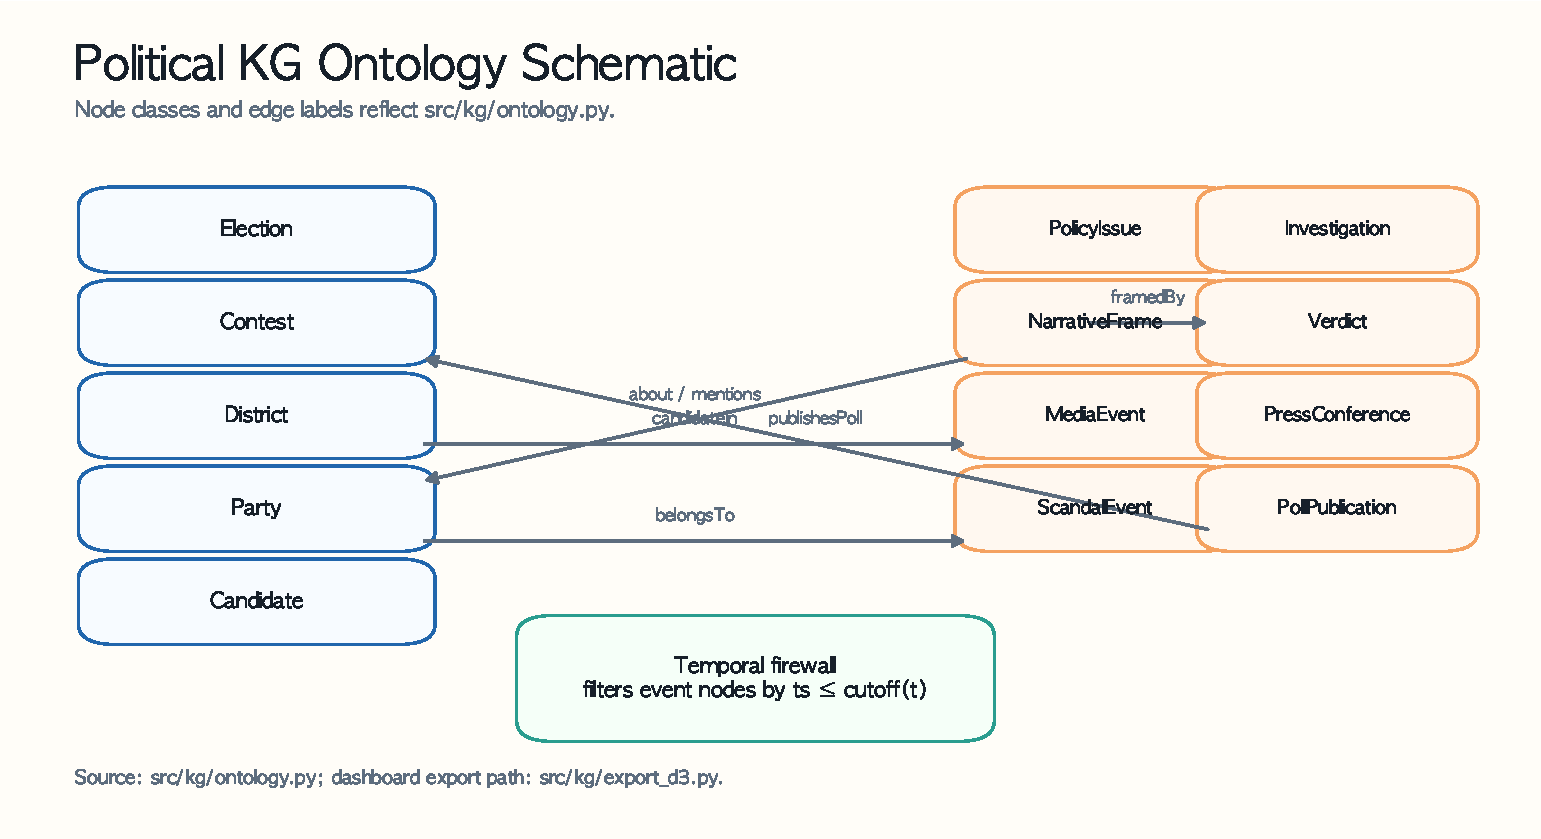
\includegraphics[width=0.94\linewidth]{assets/fig_kg_ontology_schematic.pdf}
\caption{현재 KG 온톨로지 개략도. 구조적 선거 개체는 안정적인 경선 맥락을 제공하고, 담론 개체는 시간 방화벽 아래 GraphRAG 검색이 순회하는 타임스탬프가 있는 선거운동 정보를 인코딩한다.}
\label{fig:kg-ontology-schematic}
\end{figure}

\paragraph{5개 지역 누적 통계.}
5개 목표 경선(\texttt{seoul\_mayor}, \texttt{gwangju\_mayor}, \texttt{daegu\_mayor}, \texttt{busan\_buk\_gap}, \texttt{daegu\_dalseo\_gap})을 통합한 KG는 \textbf{212개 노드와 354개 엣지}로 컴파일된다. 다섯 경선은 모두 선거일이 2026-06-03인 단일 $Election$ 노드 \texttt{election\_2026\_local}을 공유하므로, 지역 간 시점과 방화벽 컷오프 $\tau(t)$를 직접 비교할 수 있다. 클래스별 수는 $|Election|=1$, $|District|=5$, $|Contest|=5$, $|Party|=5$, $|Candidate|=17$(경선당 평균 3.4명), $|PolicyIssue|=10$, $|NarrativeFrame|=13$, $|MediaEvent|=33$, $|PressConference|=30$, $|PollPublication|=13$, $|Source|=31$, $|Person|=34$, $|CohortPrior|=15$이다. 엣지 수는 $|\texttt{about}|=61$, $|\texttt{attributedTo}|=62$, $|\texttt{framedBy}|=53$, $|\texttt{leansToward}|=45$, $|\texttt{affiliatedTo}|=34$, $|\texttt{damagesParty}|=25$, $|\texttt{candidateIn}|=17$, $|\texttt{belongsTo}|=17$, $|\texttt{mentions}|=9$, $|\texttt{speakerIs}|=9$, $|\texttt{publishesPoll}|=7$, $|\texttt{inElection}|=5$, $|\texttt{heldIn}|=5$, $|\texttt{appliesToRegion}|=5$이다. 시간 방화벽 아래 지역별 점진 공개는 서울, 광주, 대구, 부산 북구갑, 대구 달서갑 순으로 $t=0$에서 $14 / 9 / 15 / 4 / 3$개 가시 사건을 보이다가 $t=3$에서 $17 / 11 / 19 / 17 / 13$개로 증가한다.

\paragraph{정책 이슈 유형과 이슈/프레임 분리.}
10개 $PolicyIssue$ 노드는 한국 지방선거 담론을 조직하는 축에 따라 단일 주 유형을 가진다. \emph{정치}(4: 이재명 정부 중간평가, 견제 대 협력, 정부 협조, 광주의 ``김부겸 효과''), \emph{지역개발}(3: 광주형 일자리/AI 투자, 대구 신청사 건립, GTX 연장과 광역교통), \emph{이념}(1: TK 지역정체성과 변화), \emph{역사}(1: 5·18 진상규명), \emph{부동산}(1: 재개발과 주거)이다. 보완적인 13개 $NarrativeFrame$ 노드는 한동훈 대권 도전 프레임, 이진숙 불출마/국민의힘 후보 지원 프레임, 보수 블록 분열처럼 그 자체가 실체 정책 이슈는 아니지만 경선 구도를 규정하는 프레임을 포착한다. 따라서 자료는 실체 정책 축($PolicyIssue$)과 선거운동 프레이밍 축($NarrativeFrame$)이 서로 환원되지 않는다는 이중 계층 설계를 직접 뒷받침한다. KG는 시뮬레이터의 고정 입력이므로 이 수치는 sim-engineer의 후속 실행에 의해 변하지 않으며, 본 논문의 freeze 전 최종 KG 스냅샷을 나타낸다.

\subsection{문서 코퍼스와 벡터 인덱스}

뉴스 기사, 기자회견 녹취, 법원 판결문, 상세 여론조사 보고서 같은 전문 문서는 전체 배포에서는 객체 저장소에 보관되고 벡터 DB에 인덱싱될 수 있다. 현재 하네스의 P0 계약은 전체 벡터 인덱스 대신 큐레이션된 시나리오 JSON과 KG 유래 텍스트 요약을 사용하며, 저장소에는 production 벡터 인덱스가 없다. 이는 해커톤 동안 검색을 결정적으로 유지하면서도 검색 증강 생성(RAG)으로 확장할 경로를 남긴다. 시간 제약은 아래 설명대로 검색 시점에 적용된다.

\section{문제 정식화}

각 유권자가 광역단체장, 기초단체장, 지방의회 의석, 교육감 등 여러 직위에 투표할 수 있는 지방선거를 고려한다. 다음과 같이 표기한다.

\begin{itemize}
  \item $i = 1, \dots, N$: 유권자(페르소나) 인덱스.
  \item $b \in \mathcal{B}$: 투표 직위 인덱스.
  \item $k \in \mathcal{K}_b$: 직위 $b$의 후보 인덱스.
  \item $t = 0, 1, \dots, T$: 선거운동 시작부터 선거일 $T^*$까지의 시점 인덱스.
\end{itemize}

각 유권자 $i$는 사회·인구학적 속성(연령, 성별, 지역, 직업, 소득, 학력 등), 장기적 이념 위치, 기본 정당일체감 및 기타 특성을 인코딩하는 정적 맥락 벡터 $x_i$를 가지며, 합성 페르소나 자료으로부터 도출된다. 시점 $t$에서 유권자는 이슈 현저성, 후보 평가, 정부 지지, 정치 관심, 투표 성향을 요약하는 잠재 정치 상태 $z_{i,t}$를 갖는다.

시점 $t$에서 공유 정치 환경은 시점 $t$까지의 선거, 경선, 정당, 후보, 선거구, 이슈, 사건, 언론 출처, 여론조사를 인코딩하는 지식그래프 $KG_t$로 표현된다. $\mathcal{E}_t$를 $t-1$과 $t$ 사이에 발생한 새로운 사건 집합(언론 보도, 의혹 사건, 수사, 기소, 판결, 대변인 브리핑, 토론, 여론조사)으로 정의한다.

각 유권자 $i$와 시점 $t$에 대해 \emph{정보 상태} $I_{i,t}$는 지역, 언론 소비 패턴, (선택적으로) 사회 연결망 연결을 기반으로 $i$가 노출된 정치 맥락 부분을 포착하는 $KG_t$의 부분그래프로 정의된다.
\begin{equation}
I_{i,t} = \text{Subgraph}(KG_t; \text{region}(i), \text{media\_diet}_i, \text{social\_links}_i).
\end{equation}

모형화 목표는 $(x_i, z_{i,0}, \{KG_t\}_{t=0}^T)$를 각 유권자 $i$와 직위 $b$에 대해 다음에 매핑하는 과정을 정의하는 것이다.

\begin{itemize}
  \item 투표 결정 $V_i \in \{0,1\}$ (투표/기권).
  \item $V_i = 1$이면 비밀 투표 선택 $y_{i,b} \in \mathcal{K}_b$.
\end{itemize}

유권자에 걸쳐 집계하면 각 투표 직위에 대해 원하는 집계 수준(예: 선거구, 시, 도)에서 예측 투표율과 득표율을 얻는다.

\section{모형}

\subsection{KG 증강 정보를 갖는 유권자 효용}

유권자 $i$, 직위 $b$, 후보 $k$에 대해 시점 $t$의 잠재 효용을 다음 형태로 가정한다.
\begin{equation}
U_{i,b,k}(t) = U^{\text{base}}_{i,b,k} + \Delta U^{\text{media}}_{i,b,k}(I_{i,t}) + \Delta U^{\text{poll}}_{i,b,k}(t) + \Delta U^{\text{gov}}_{i,b,k}(t) + \varepsilon_{i,b,k}(t),
\end{equation}
여기서 $\varepsilon_{i,b,k}(t)$는 특이 오차항이다.

기본 효용은 유권자와 후보 간 구조적 정렬을 인코딩한다.
\begin{equation}
U^{\text{base}}_{i,b,k} = \beta_b^\top f(x_i, c_{b,k}),
\end{equation}
여기서 $c_{b,k}$는 후보·정당 속성(정당 라벨, 이념, 현직 여부, 경력, 지역 연고)을 모으고, $f$는 상호작용(예: 이념 거리, 정당일체감, 사회·인구학적 일치)을 포착하는 특징 매핑이다.

정보 의존 성분 $\Delta U^{\text{media}}_{i,b,k}(I_{i,t})$와 $\Delta U^{\text{poll}}_{i,b,k}(t)$는 각각 KG에서 도출된 정보 상태와 공표 여론조사 노출 신호의 함수다. 보류된 공식 여론조사 label은 별도 노출 ablation을 선언하지 않는 한 유권자의 정보 상태 밖에 둔다.

\subsection{언론, 의혹 사건, 법적 사건}

시점 $t$까지 후보 $k$에 영향을 주는 언론·법적 사건은 $I_{i,t}$로부터 도출된 valence 충격으로 모형화한다. $\mathcal{E}^{\text{scandal}}_{i,k,t}$를 $I_{i,t}$에 존재하는 $k$ 대상 의혹 사건 관련 사건 집합이라 하자. 각 사건 $e$는 심각도, 신뢰성, 발생 시점 $t_e$ 같은 속성을 갖는다.

누적 언론 기여는 다음과 같이 정의한다.
\begin{equation}
\Delta U^{\text{media}}_{i,b,k}(I_{i,t}) = \sum_{e \in \mathcal{E}^{\text{scandal}}_{i,k,t}} \alpha^{\text{scandal}}_b \, s(e) \, \exp(-\lambda^{\text{scandal}} (t - t_e)) \, h_i(e),
\end{equation}
여기서 $s(e)$는 사건 $e$의 심각도와 신뢰성을 인코딩하고, $\lambda^{\text{scandal}}$은 시간 감쇠를 통제하며, $h_i(e)$는 유권자별 민감도(언론 신뢰, 정치 관심, 사전 태도)를 포착한다. 유사한 구성은 긍정 valence 사건(지지 선언, 성과 등)과 주로 이슈 현저성·프레임에 영향을 미치는 사건에도 사용할 수 있다.
의혹 사건의 salience는 시간 감쇠와 선거 근접성 가중치를 함께 적용하는데, 이는 정부 스캔들 보도가 선거가 가까워질수록 증가한다는 근거를 반영한다~\cite{garz2019scandals}.

\subsection{여론조사 피드백}

$\hat p_{b,k}(t)$를 시점 $t$에서 직위 $b$의 후보 $k$ 통합 여론조사 지지율, $\bar{p}_b(t)$와 $p_{\min,b}(t)$를 직위 $b$ 후보들 사이 평균과 최소 지지율이라 하자. 편승효과와 약세효과 반응을 포착하기 위해 다음과 같이 정의한다.
\begin{equation}
\Delta U^{\text{poll}}_{i,b,k}(t) = \eta^{\text{bw}}_{i,b} \, \big(\hat p_{b,k}(t) - \bar{p}_b(t)\big)_+ + \eta^{\text{ud}}_{i,b} \, \big(p_{\min,b}(t) - \hat p_{b,k}(t)\big)_+,
\end{equation}
여기서 $(x)_+ = \max(x,0)$이며, $\eta^{\text{bw}}_{i,b}$와 $\eta^{\text{ud}}_{i,b}$는 유권자·직위별 편승효과와 약세효과 민감도다.

여론조사 피드백은 공표된 여론조사 노출 이후 다수 선택지가 추가 표를 얻었다는 온라인 투표 실험 근거에 따라 bounded bandwagon prior로 모형화한다~\cite{farjam2021bandwagon}. 다단계 또는 반복 정보 설정에서는 여론조사 공개가 뒤처진 후보를 두드러지게 만들 때 약세효과 반응도 허용한다~\cite{morton2020underdog}. 이 모수는 유권자 유형(강한 당파주의자 대 약한 식별자 대 무당층)과 직위 유형(지방 행정 대 지방 의회)에 따라 달라질 수 있으며, 그 추정은 과거 여론조사 및 선거 데이터에 의존한다. 기본 validation 및 counterfactual 모드에서 $\hat p_{b,k}(t)$는 scoring/보정 객체이고, prompt에는 명시적 공표 여론조사 사건 또는 내생적 모의응답 요약만 들어간다.

\subsection{정부 지지율과 이차 효과}

$G(t)$를 기준 수준 $\bar{G}$ 주변으로 정규화된 시점 $t$의 전국 정부 또는 대통령 지지율이라 하자. 여당 후보에 대해 이차 선거 항을 도입한다.
\begin{equation}
\Delta U^{\text{gov}}_{i,b,k}(t) = \zeta_b \, g_i \, (G(t) - \bar{G}) \, \mathbb{I}[\text{party}(k) = \text{incumbent}],
\end{equation}
여기서 $\zeta_b$는 직위 $b$에 대한 전국 지지율의 영향을 조정하고, $g_i$는 저주목 선거에서 유권자 $i$가 정부를 보상하거나 처벌하는 경향을 측정하며, $\mathbb{I}[\cdot]$는 지시함수다.

\subsection{투표 결정}

유권자 $i$의 투표 결정은 잠재 투표 성향 함수에 의해 결정된다.
\begin{equation}
\Theta_i(t) = \gamma^\top q(x_i, z_{i,t}, G(t), I_{i,t}),
\end{equation}
여기서 $q$는 정치 관심, 인지된 선거 중요도, 정부에 대한 불만, 투표 비용, $I_{i,t}$ 내 현저한 사건 같은 예측 변수를 포함한다. 투표 지시자는 다음과 같다.
\begin{equation}
V_i = \mathbb{I}[\Theta_i(T^*) + \xi_i > 0],
\end{equation}
$\xi_i$는 모형화되지 않은 충격을 포착한다.

\subsection{다중 투표에 걸친 상관 선택}

분할·일관투표 패턴을 포착하기 위해 모형은 잠재 요인을 직위 간에 공유한다. $p_i$를 정당일체감, $l_i$를 이념 위치, $r_i$를 정부 평가라 하자. 이 요인은 다음을 통해 모든 기본 효용 $U^{\text{base}}_{i,b,k}$에 들어간다.
\begin{equation}
U^{\text{base}}_{i,b,k} = \beta_b^\top f(x_i) + \phi_b \, \text{PartyAffinity}(p_i, \text{party}(k)) + \psi_b \, \text{IdeologyDistance}(l_i, l_{b,k}) + \dots,
\end{equation}
이로써 직위 간 선택은 공유 잠재 특성을 통해 상관되며, 동시에 직위별 모수($\beta_b, \phi_b, \psi_b$)와 특이 오차가 분할투표를 생성할 수 있게 한다.

\subsection{LLM 에이전트를 통한 비밀 투표}

시뮬레이션에서 각 유권자 에이전트는 페르소나의 정적 속성을 시스템 프롬프트에 인코딩하고 $I_{i,t}$로부터 도출된 현재 정치 상태를 user prompt에 요약하는 LLM 기반 커스텀 에이전트로 구현된다. 선거 시점 $T^*$에서 에이전트는 한국 투표용지를 모방하고 투표의 비밀성을 강조하는 프롬프트를 받는다.

\begin{itemize}
  \item 모든 직위 후보를 나열하고 사퇴자는 무자격으로 표시한다.
  \item 선택은 비밀이며 공유되지 않음을 명시한다.
  \item 먼저 투표 여부를 결정하고, 투표한다면 직위별로 정확히 한 명의 자격 후보를 선택하도록 지시한다.
\end{itemize}

보정에는 표본 잡음 감소를 위해 결정적 디코딩(예: greedy)을 사용하거나 불확실성 추정을 위해 에이전트당 여러 표본을 사용할 수 있다. LLM 기반 결정은 위 효용 프레임워크와 결합되며, 효용을 LLM 출력의 잠재 설명으로 다루거나 LLM을 사용하여 선택 확률을 근사할 수 있다.

\section{시스템 아키텍처}

\subsection{다중 에이전트 엔진: LLMPool 기반 유권자 에이전트}

다중 에이전트 엔진은 모든 LLM 호출을 다중 provider 추상화 계층인 LiteLLM(\texttt{litellm>=1.50})을 통해 보내는 얇은 커스텀 유권자 에이전트 계층을 사용한다. LiteLLM은 모형 prefix 문자열에 따라 Gemini, OpenAI, Anthropic, Azure OpenAI, Vertex AI, AWS Bedrock, Groq, OpenRouter 등으로 요청을 라우팅한다. 기본 개발 설정은 thinking을 끈 JSON-object 응답의 \texttt{gemini/gemini-3.1-flash-lite-preview}이며, provider 전환은 \texttt{LITELLM\_MODEL} 환경변수 변경만으로 가능하다. provider 비의존 \texttt{LLMPool}은 LiteLLM 앞에서 API 키를 회전하고, 키별 rolling RPM 제한을 적용하며, 429 및 일시적 네트워크 오류에 retry/backoff를 수행하고, 메시지·모형·생성 설정 해시에 의해 키가 정해지는 SQLite 캐시에 응답을 저장한다. CAMEL(\texttt{camel-ai>=0.2.90})은 framework 관리 에이전트 상태, 다중 에이전트 society, 도구 호출 orchestration이 필요한 경우를 위한 선택적 Plan B 계층으로 유지된다~\cite{li2023camel}. 핵심 구성요소는 다음과 같다.

\begin{itemize}
  \item \textbf{VoterAgent}: 페르소나별 시스템 프롬프트, 호출별 모형 라우팅, JSON 파싱, retry 회계, KG 요약 접근권을 가진 커스텀 LLM 유권자 래퍼.
  \item \textbf{ElectionEnvironment}: 시간 단계 조율, 사건 적용, 효용 갱신, 투표 트리거.
  \item \textbf{KGService}: 각 에이전트에 대한 관련 부분그래프와 텍스트 요약을 검색하는 API 질의 제공.
\end{itemize}

각 시간 단계에서 환경은 새 사건으로 $KG_t$를 갱신하고, KG 서비스를 호출해 각 에이전트(또는 대표 클러스터)에 대해 $I_{i,t}$를 구성하며, 효용을 갱신하고 선택적으로 제한된 사회적 상호작용을 허용한다. $T^*$에서 비밀 투표 프롬프트가 발행되고 응답이 집계된다.

\subsection{시간적 정보 방화벽}

선거 후 지식이 과거 시뮬레이션으로 누출되는 것을 막기 위해 본 프레임워크는 \texttt{src/kg/firewall.py}에 구현된 시간적 정보 방화벽을 사용한다. 시뮬레이션 시점 $t \in \{0, \dots, T-1\}$와 선거운동 구간 $[t_{\text{start}}, t_{\text{end}}]$가 주어지면, 방화벽은 $t$를 벽시계 컷오프로 변환한다.
\begin{equation}
\tau(t) = t_{\text{start}} + \frac{t}{T-1}\big(t_{\text{end}} - t_{\text{start}}\big),
\end{equation}
그리고 타임스탬프가 $\tau(t)$를 넘지 않는 사건으로 검색을 제한한다.
\begin{equation}
\mathcal{R}(p, t) = \big\{ e \in \mathcal{E} : \mathrm{ts}(e) \le \tau(t) \big\},
\end{equation}
여기서 $p$는 질의하는 페르소나이고 $\mathcal{E}$는 KG의 전체 사건 집합이다. 추가 제약은 다음과 같다.

\begin{itemize}
  \item 에이전트 프롬프트는 모형이 제공된 정보에만 근거해 결정하고 미래 사건을 추측하지 않도록 명시적으로 지시한다.
  \item 기본 LLM은 실험 전반에 걸쳐 고정되며, 이용 가능한 정보의 변화는 오로지 방화벽과 데이터 슬라이스를 통해 통제된다.
  \item \texttt{src/kg/firewall.py}의 7개 단위 테스트는 단조성(\,$\mathcal{R}(p,t) \subseteq \mathcal{R}(p,t')$ for $t \le t'$), $t=T-1$ 경계 포함, 위상적으로 도달 가능하더라도 $\mathrm{ts}(e) > \tau(t)$인 사건의 제외 같은 불변식을 고정한다. 2026-04-25 컷오프의 5개 지역 시드도 회귀 테스트로 쓰이며, 작성 시점 기준 PASS 상태다.
  \item 종단 간 검증으로 시뮬레이터는 투표 결정 동안 검색된 \texttt{kg\_events\_used} 집합을 지역별로 기록한다. KG 대시보드 스냅샷은 목표 순서의 5개 지역에서 가시 사건 수가 $t=0$의 $\{20, 14, 16, 11, 9\}$에서 $t=3$의 $\{22, 14, 18, 14, 14\}$로 단조 증가함을 보여준다. 에이전트 맥락에는 어떤 시점에서도 $\mathrm{ts}(e) > \tau(t)$인 사건이 나타나지 않아 실제 검색 경로에서 방화벽이 강제됨을 확인한다.
\end{itemize}

\begin{figure}[t]
\centering
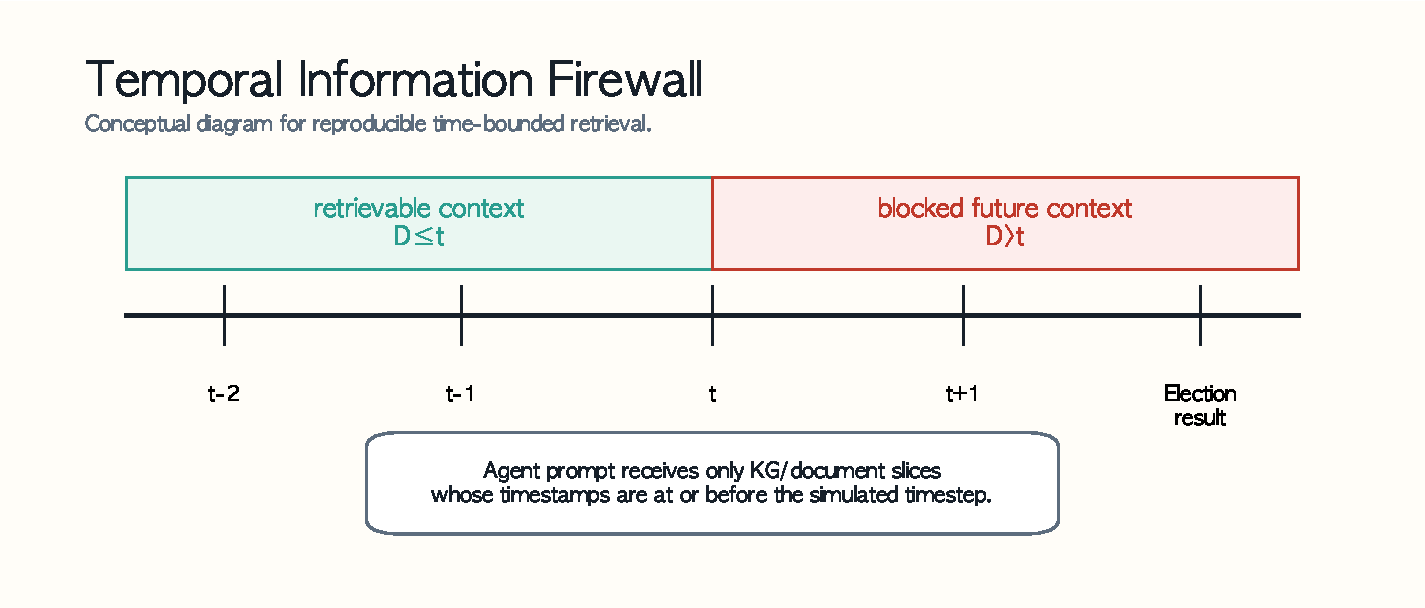
\includegraphics[width=0.88\linewidth]{assets/fig_temporal_firewall.pdf}
\caption{시간적 정보 방화벽. 각 시점은 벽시계 컷오프 $\tau(t)$에 매핑되며, 검색은 위상적으로 도달 가능하더라도 그 컷오프 이후의 타임스탬프를 갖는 사건을 제외한다.}
\label{fig:temporal-firewall}
\end{figure}

이 설계는 모호할 수 있는 LLM의 보고된 지식 컷오프에만 의존하는 것보다 신뢰성이 높으며, 시뮬레이션 정보 집합을 역사 기록과 정렬한다.

\subsection{시각화 및 분석 계층}

시뮬레이션 엔진 위에 하네스는 계획된 Streamlit 시각화 계층을 정의한다. Docker 런타임에는 필요한 Python 대시보드 의존성과 \texttt{ui/dashboard/app.py}를 기대하는 \texttt{docker compose} 대시보드 profile이 포함되어 있지만, 현재 저장소 스냅샷에는 \texttt{ui/} 구현이 없다. 의도된 시각화 계층은 다음을 노출한다.

\begin{itemize}
  \item 선거구·직위별 투표율과 득표율의 인터랙티브 지도.
  \item 후보, 이슈, 사건, 언론 매체 간 관계를 보여주는 KG 기반 뷰와 선거운동 동학 탐색용 시간 슬라이더.
  \item 집계된 페르소나 통계(인구통계 분포, 이슈 관심사) 및 시나리오별 진화.
\end{itemize}

이 뷰는 모형 진단과 실질적 정치 분석을 모두 지원한다.

\section{실험 설계}

\subsection{학습·검증·테스트 분할}

PolitiKAST의 핵심 실증 요구사항은 2026년 선거 결과를 주장하기 전에 보류된 공식 여론조사 목표를 먼저 재현하는 것이다. 이 단계가 없으면 현재 선거 실행은 실제 후보 이름 위에서 수행되는 zero-shot LLM 시뮬레이션에 가깝다. 따라서 다음 rolling-origin 분할을 사용한다.

\begin{itemize}
  \item \textbf{과거 훈련 자료}: 기본 효용, 투표율, 여론조사 피드백, 정부 지지율 모수를 초기화하는 과거 한국 선거 및 여론조사 시계열.
  \item \textbf{현재 선거 보정 구간}: 2025-12-03 이후 특정 cutoff $\tau_v$까지 등록된 2026 지방선거 공식 여론조사.
  \item \textbf{현재 선거 검증 구간}: $\tau_v$ 이후 조사 또는 공표된 공식 여론조사. 해당 결과는 모형 산출 이후에만 scoring에 사용한다.
  \item \textbf{최종 선거 검정}: 2026년 실제 득표율과 당선자. 이는 여론조사 검증 gate를 통과한 뒤에만 사용한다.
\end{itemize}

각 검증 대상 여론조사 $r$에 대해, evaluator는 해당 조사 기간 또는 최초 공표 시점 직전 cutoff $\tau_r^-$까지의 여론조사 아카이브와 통합 시계열을 유지한다. 그러나 유권자 에이전트는 그 시점까지 공개된 KG 사건과 공개 정보만 받으며, 보류된 consensus 값 자체는 prompt에 들어가지 않는다. 이후 동일한 경선·후보군·날짜 bucket에 대해 $P^{\text{model-poll}}_{r,b,k}$를 생성하고, 보류된 공식 여론조사 $\hat p_{r,b,k}$와 비교한다. 이렇게 해야 같은 여론조사가 입력 신호와 검증 label로 동시에 쓰이는 누수를 막을 수 있다.

\subsection{모수 추정}

모수 벡터 $\theta$는 기본 효용 계수($\beta_b, \phi_b, \psi_b$), 언론 감쇠 및 강도 모수($\alpha^{\text{scandal}}_b, \lambda^{\text{scandal}}$), 여론조사 피드백 계수($\eta^{\text{bw}}_{\cdot,\cdot}, \eta^{\text{ud}}_{\cdot,\cdot}$), 정부 지지율 항($\zeta_b$), 투표 모수($\gamma$)를 포함한다. 실무적으로는 차원을 줄이기 위해 유권자 유형이나 지역으로 묶을 수 있다.

\textbf{여론조사 보정 및 검증.} 과거 및 현재 선거 보정 구간의 통합 여론조사를 사용하여 시뮬레이션과 관측 여론조사 지지율 간 차이를 측정하는 손실 함수를 최소화한다. 예를 들어
\begin{equation}
\mathcal{L}_{\text{poll}}(\theta) = \sum_{j,t,b,k} w_{j,t} \Big(P^{\text{model-poll}}_{j,b,k}(t; \theta) - \hat p_{j,b,k}(t)\Big)^2,
\end{equation}
여기서 $j$는 선거 또는 지역, $w_{j,t}$는 중요도 가중치다. 보류된 현재 선거 여론조사는 같은 정의로 scoring하되 모수 업데이트에는 사용하지 않는다. 원시 여론조사는 조사기관 이질성에 대한 견고성 점검과 통합 smoothing이 체계적 오차를 숨기지 않는지 확인하기 위해 보존된다.

\textbf{검증 이후 선거 검정.} 여론조사 검증 gate 이후 모수를 고정한 채 전체 선거를 시뮬레이션하고, 집계 산출 $V^{\text{model}}_{j,b,k}(T^*; \theta)$를 실현 득표율 $V^{\text{real}}_{j,b,k}$와 RMSE, MAE, 승자 정확도, 스윙 탐지 같은 지표로 비교한다. 이 최종 검정은 선거일 이전에는 존재하지 않으며, 본 초안에서 주장하지 않는다.

\subsection{보정 이후 반사실적 inference}

본 프로젝트의 실제 inference 단계는 보정·검증 이후 시작된다. 설정 $\theta^\star$와 KG retrieval 정책을 동결한 뒤, 후보 사퇴, 공천 결과, 지지 선언, 논란, 토론 같은 사건열 $\Delta KG_s$를 기준 시나리오 $s$에 주입한다. 유권자 에이전트는 같은 페르소나 표본과 model routing, 숨겨진 여론조사 label 규칙 아래에서 $KG_{\le t} \cup \Delta KG_{s,\le t}$를 보고 다시 실행된다. 이 산출물은 \texttt{target\_series=counterfactual\_prediction}으로 표기되며, train/validation label이나 예측 정확도의 근거가 아니다.

구현상 intervention은 \path{_workspace/data/interventions/<region>/} 아래 JSON 파일로 저장한다. 각 파일은 후보 patch, 사건 patch, factual premise의 source URL, 동결 profile(\texttt{calibration\_profile})을 포함한다. 결과 JSON은 \texttt{meta.counterfactual}에 \texttt{intervention\_id}, \texttt{base\_scenario\_id}, \texttt{frozen\_params}, \texttt{poll\_targets\_visible\_to\_agents=false}, 선택적 \texttt{delta\_vs\_baseline}을 기록한다.

\subsection{계산 제약과 부분 표본}

수십만~수백만 에이전트로 전체 시뮬레이션을 실행하는 것은 LLM 호출이 관련될 때 특히 계산적으로 비싸다. 제한된 시간과 예산(예: 12시간 해커톤)을 수용하기 위해 다음을 제안한다.

\begin{itemize}
  \item 실험을 일부 지역으로 제한(예: 한 광역시와 몇 개 자치구).
  \item 지역당 페르소나 수 제한(예: 5,000~10,000)하면서 계층 표본 추출로 인구통계 비율 보존.
  \item 단순화된 시간 격자 사용(예: 선거운동 초기, 중기, 후기, 선거일의 4개 핵심 시점).
  \item 일부 갱신(예: 언론 및 여론조사 효과)을 LLM 호출 없이 해석적으로 근사하고, LLM 추론은 최종 투표 선택에만 보존.
\end{itemize}

이러한 설계 선택은 모형 명세와 보정의 빠른 반복을 허용하면서도 더 큰 규모 시뮬레이션으로 가는 경로를 유지한다.

\subsection{현재 해커톤 목표 경선}

현재 하네스는 일반 정식화를 서로 다른 정치 레짐과 시나리오 유형을 점검하도록 선택된 5개 목표 경선으로 좁힌다. 표~\ref{tab:target-contests}는 활성 목표를 요약한다. 지역별 표본 수는 Gemini API capacity probe 이후 정책 계층이 결정한다.

\begin{table}[h]
\centering
\caption{현재 PolitiKAST 하네스의 목표 경선. 지역별 표본 $n$은 Gemini API capacity probe 이후 정책 계층이 설정한다(부록~\ref{app:capacity}); \texttt{TBD} 값은 실험 시점에 채운다.}
\label{tab:target-contests}
\small
\begin{tabular}{p{0.18\textwidth}p{0.18\textwidth}p{0.42\textwidth}p{0.10\textwidth}}
\toprule
지역 식별자 & 경선 유형 & 선정 근거 & 표본 $n$ \\
\midrule
\texttt{seoul\_mayor} (서울) & 광역단체장 & 전국 기준선; 주목도 높은 광역 경선 & TBD \\
\texttt{gwangju\_mayor} (광주) & 광역단체장 & 진보 우세 기준선; 이념 대비 & TBD \\
\texttt{daegu\_mayor} (대구) & 광역단체장 & 보수 우세 기준선; 이념 대비 & TBD \\
\texttt{busan\_buk\_gap} (부산 북구갑) & 국회의원 보궐선거 & ``미니 총선'' 대표 사례: 한동훈(무소속, 전 PPP 대표) vs. 하정우(무소속/대통령실 AI 수석, 민주당 영입 추진 대상) vs. 박민식(PPP). 비게 된 DPK 보유 지역구에서 후보 정체성과 정당 레이블 효과를 분리한다. & TBD \\
\texttt{daegu\_dalseo\_gap} (대구 달서갑) & 국회의원 보궐선거 & 조건부 보수 강세 시나리오: 유영하가 대구시장 출마로 달서갑을 비우는 경우 서재헌(DPK) vs. 국민의힘 단일 후보 proxy 홍성주. 김민수는 비활성 전략공천설 맥락으로만 남기고, 이진숙은 2026-04-25 대구시장 불출마 및 국힘 후보 지원 선언 이후 후보군에서 제외한다. & TBD \\
\bottomrule
\end{tabular}
\end{table}

두 보궐선거 사례는 의도적으로 상보적이다. 부산 북구갑은 전 여당 대표가 무소속으로 출마하고 민주당 영입 압박을 받는 대통령실 AI 수석을 무소속 후보로 모델링하는 고정보 ``미니 총선''으로, 강한 언론 노출 아래 PolitiKAST가 움직임을 후보 정체성과 정당 레이블 중 어디에 귀속하는지 직접 점검한다. 대구 달서갑은 정반대 구조, 즉 단일 DPK 도전자와 PPP 내부 분열이 맞서는 보수 강세 지역으로, 우세 정당 내부의 조정 실패를 모형이 포착하는지 살핀다. 5개 지역의 Nemotron-Personas-Korea 커버리지는 성인 페르소나 기준 $185{,}228 / 27{,}594 / 46{,}934 / 5{,}421 / 10{,}617$명이고 평균 연령은 $49.13 / 49.58 / 51.25 / 52.48 / 50.61$세다. 이는 capacity에 의해 제한되는 실제 표본보다 훨씬 큰 층화 표본 기반을 제공한다.

\begin{figure}[t]
\centering
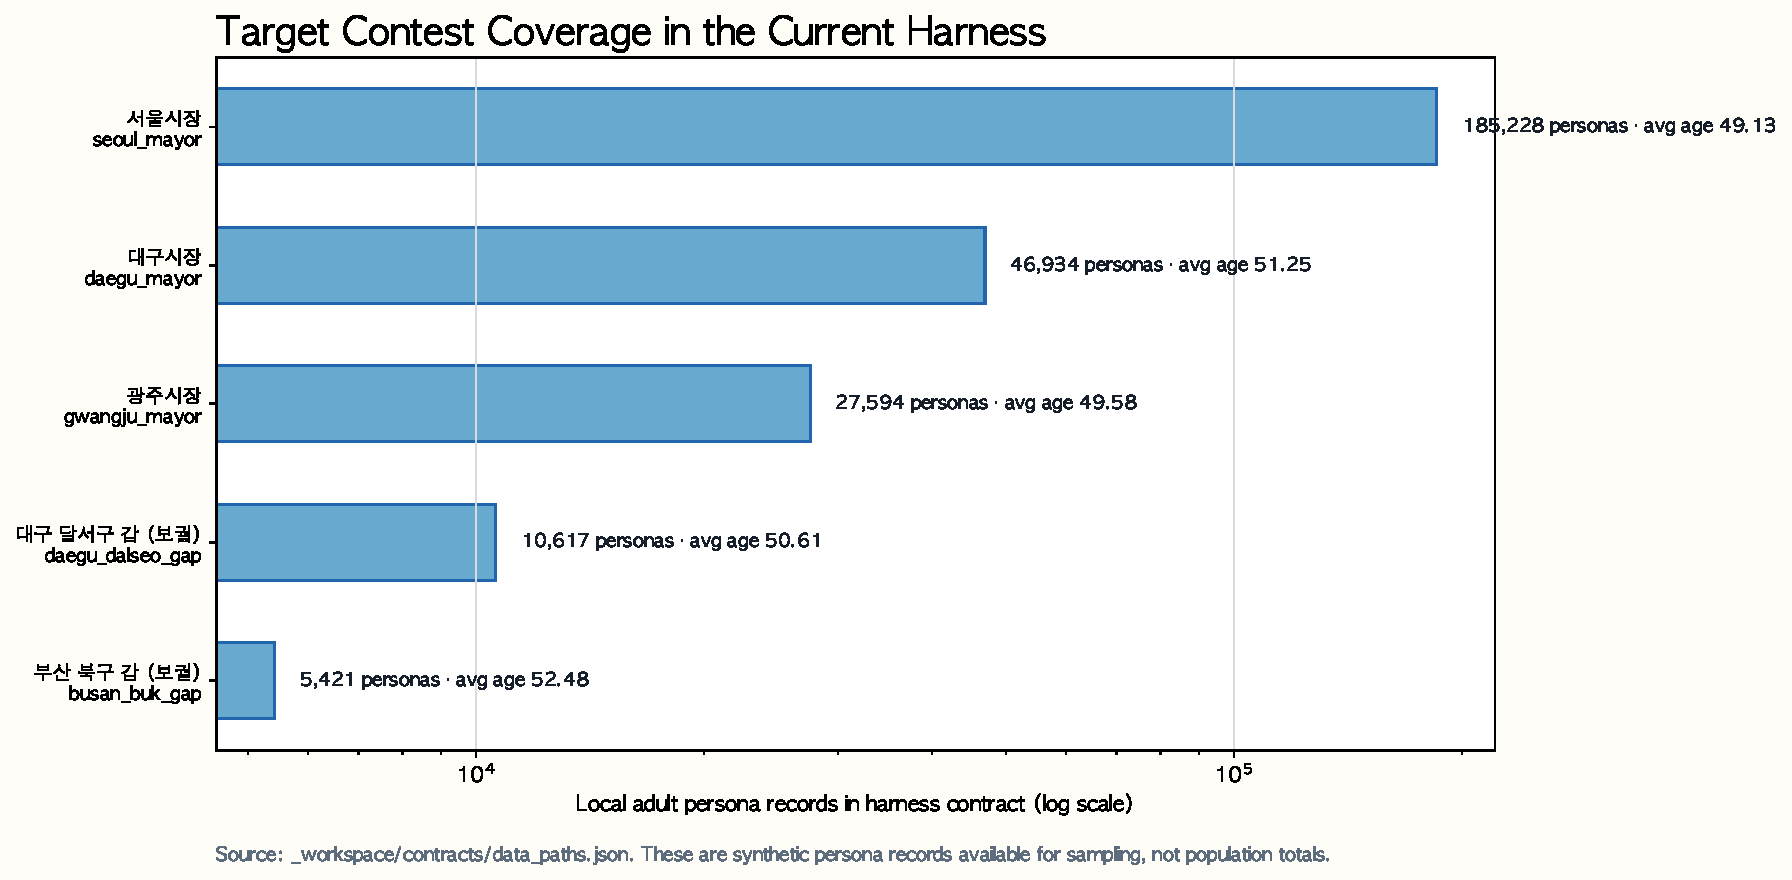
\includegraphics[width=0.92\linewidth]{assets/fig_target_region_coverage.pdf}
\caption{현재 5개 목표 경선의 성인 페르소나 커버리지. 수와 평균 연령은 하네스가 사용하는 로컬 Nemotron-Personas-Korea 샤드에서 온 것이며, 최종 실험 표본 수가 아니라 표본 추출 기반을 정의한다.}
\label{fig:target-region-coverage}
\end{figure}

\section{검증 프로토콜 및 하네스 진단}
\label{sec:results}

본 절은 검증 프로토콜과 하네스 진단이며, 보정된 2026년 선거 예측이 아니다. 현재 로컬 증거에는 \texttt{\_workspace/snapshots/results/seoul\_mayor\_\_smoke.json}에 기록된 \texttt{seoul\_mayor\_\_smoke} 스키마 인제션 스모크 실행이 있다. 이 실행은 보정된 선거 예측이 아니라 하네스 점검이다. 20개 페르소나, 2개 시점, 3개 자리표시자 후보를 사용하며 \texttt{kg\_events\_used}에는 KG 사건이 없다.

\texttt{\_workspace/snapshots/results\_index.json}은 서울 스모크 실행 외에도 \texttt{\_workspace/snapshots/results/} 아래 목표 경선 산출물을 색인한다. 이 산출물은 보정된 예측이나 외부 검증 선거 예측이 아니라 로컬 하네스 출력이다. 또한 policy log는 v1.4 실행이 높은 SQLite cache 재사용과 불완전한 key rotation 때문에 deterministic vote-share sweep을 만든 것으로 invalidation 처리한다. 따라서 현재 득표율 필드는 공식 여론조사 검증 실행이 cache 상태, key 수, 검증 label과 함께 기록될 때까지 공학적 진단으로만 사용한다.

Sim-engineer는 후속 표와 그림이 의존하는 결과 스키마(\texttt{result\_schema.json})를 다음과 같이 고정한다. \texttt{final\_outcome.\{turnout, vote\_share\_by\_candidate, winner\}}, \texttt{poll\_trajectory[].\{date, support\_by\_candidate, turnout\_intent, consensus\_var\}}, \texttt{demographics\_breakdown.\{by\_age\_group, by\_education, by\_district\}}, \texttt{virtual\_interviews[]}, \texttt{kg\_events\_used[]}이다. 현재 JSON 산출물도 \texttt{features}, \texttt{concurrency}, timestamp, \texttt{voter\_stats.\{calls, parse\_fail, abstain\}}를 포함한 \texttt{meta} 블록을 가진다.

\begin{table}[h]
\centering
\caption{\texttt{seoul\_mayor\_\_smoke} 스모크 실행 결과. 값은 로컬 결과 산출물에서 복사했으며 보정된 예측 성능으로 해석하지 않는다.}
\label{tab:smoke-result}
\small
\begin{tabular}{ll}
\toprule
항목 & 값 \\
\midrule
지역 / 경선 & \texttt{seoul\_mayor} / \texttt{seoul\_mayor\_2026} \\
페르소나 / 시점 & 20 / 2 \\
활성 기능 & bandwagon, KG retrieval, second-order, underdog \\
동시성 & 8 \\
여론 궤적 & $t=0$: A 68.42\%, B 31.58\%, C 0.00\%; $t=1$: A 75.00\%, B 25.00\%, C 0.00\% \\
최종 산출 & A 84.21\%, B 15.79\%, C 0.00\%; 승자 \texttt{cand\_A} \\
투표율 / 기권 & 95.00\% / 1 \\
LLM 응답 통계 & 63 calls, 0 parse failures, 2 abstain decisions \\
사용된 KG 사건 & 0 \\
\bottomrule
\end{tabular}
\end{table}

\begin{table}[h]
\centering
\caption{현재 색인된 로컬 하네스 산출물. 득표율은 \texttt{final\_outcome.vote\_share\_by\_candidate}에서 복사했으며 보정된 예측 성능으로 해석하지 않는다.}
\label{tab:local-harness-results}
\small
\begin{tabular}{lrrllr}
\toprule
지역 & $n$ & $T$ & 승자 필드 & 최종 득표율 & 파싱 실패 \\
\midrule
광주광역시장 & 20 & 1 & \texttt{c\_gwangju\_dpk} & 35.29 / 23.53 / 11.76 / 29.41 & 0 \\
대구광역시장 & 20 & 1 & \texttt{c\_daegu\_ppp\_choo} & 52.63 / 10.53 / 15.79 / 21.05 & 0 \\
부산 북구갑 & 20 & 1 & \texttt{c\_busan\_dpk} & 55.56 / 22.22 / 22.22 & 0 \\
대구 달서갑 & 20 & 1 & \texttt{c\_dalseo\_dpk} & 31.58 / 15.79 / 31.58 / 21.05 & 0 \\
서울시장 & 5 & 1 & \texttt{c\_seoul\_dpk} & 0.00 / 0.00 / 0.00; 전원 기권 & 30 \\
\bottomrule
\end{tabular}
\end{table}

\begin{figure}[t]
\centering
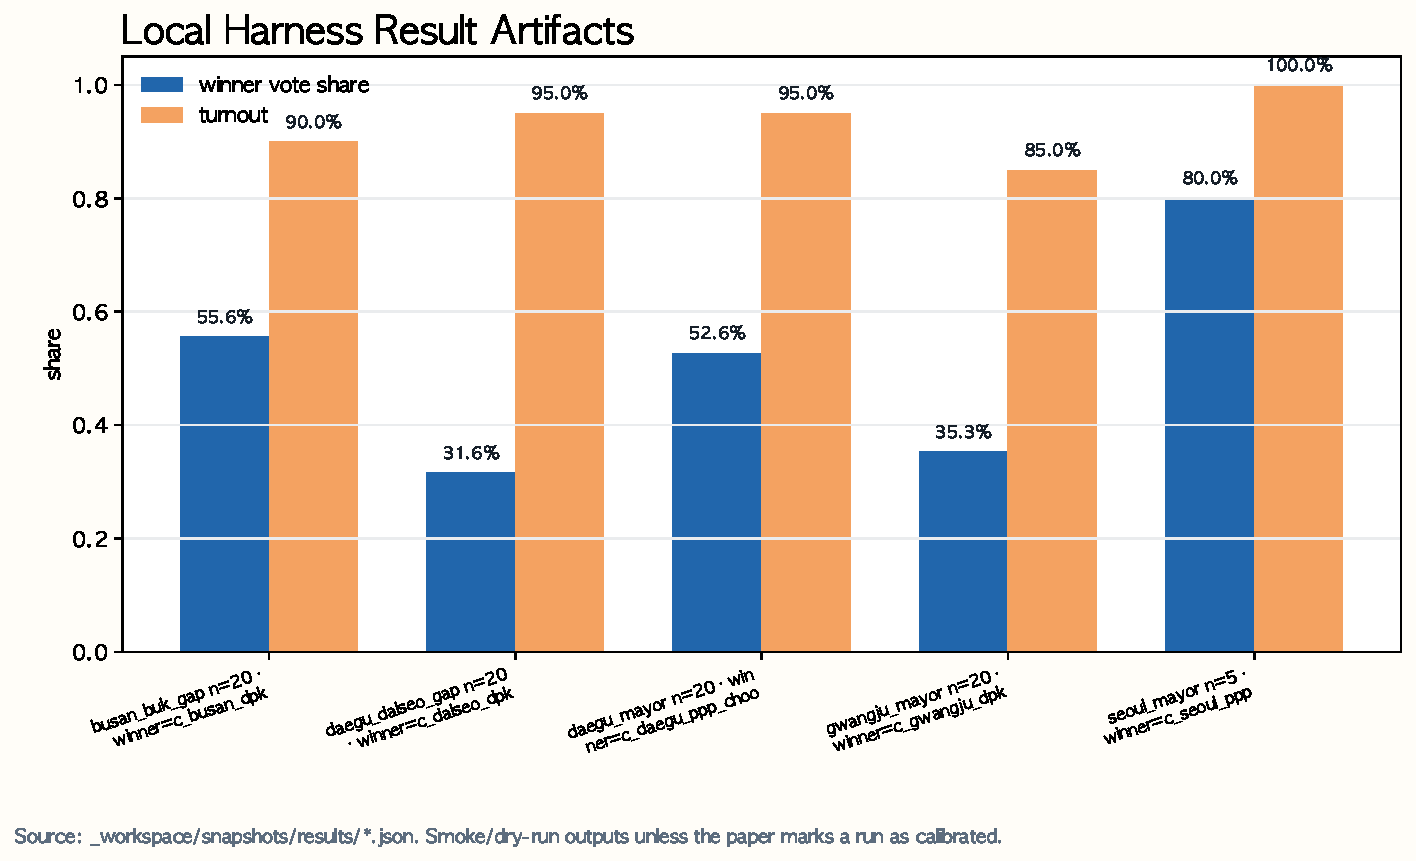
\includegraphics[width=0.94\linewidth]{assets/fig_local_result_artifacts.pdf}
\caption{현재 색인된 로컬 결과 산출물. 막대는 로컬 JSON 출력에 이미 존재하는 필드만 시각화하며, 보정된 예측이나 외부 검증 선거 예측이 아니라 하네스 진단으로 읽어야 한다.}
\label{fig:local-result-artifacts}
\end{figure}

\subsection{정성 예시: 가상 인터뷰}
\label{sec:qual-example}

하네스는 집계 여론 궤적 외에도 각 LLM 유권자 에이전트가 방금 내린 선택을 설명하는 가상 인터뷰 transcript를 생성한다. \texttt{gemini/gemini-3-flash-preview}(Gemini 3 Flash preview)를 사용한 서울 첫 live run은 일반적인 AI 문체가 아니라 페르소나에 가까운 transcript를 생성했다. 예를 들어 서울에 거주하는 50세 여성 사무직 유권자가 오세훈(People Power Party)에게 투표한 뒤 다음과 같이 설명했다.

\begin{quote}
\itshape
``서류 일은 복잡해서 딱 질색인데, 그저 지금처럼 서울시 살림을 안정적으로 잘 해줄 사람이 누구인지를 보게 되네요.''
\end{quote}

\noindent 이 응답의 \texttt{key\_factors} 필드는 ``시정 안정성'', ``후보의 행정 경험'', ``평범한 가족생활의 지속성''을 나열한다(부록~\ref{app:eq-code}). 이는 추상적 정책 문구라기보다 Nemotron-Personas-Korea의 \texttt{family\_persona}와 \texttt{professional\_persona} 서사에 그럴듯하게 연결된다. 이 단일 transcript는 예측 정확도의 증거가 아니다. 해당 live run은 $n{=}5$로 추론 기준에 훨씬 못 미친다. 다만 prompt와 JSON schema 설계가 Phase 3 전체 실행 이후 정성 분석에 쓸 수 있는 유권자 에이전트 출력을 만든다는 점을 보여준다.

검증 acceptance criteria는 다음과 같다.

\begin{itemize}
  \item 공식 NESDC 여론조사 registry를 \texttt{raw\_poll}, \texttt{raw\_poll\_result}, \texttt{poll\_consensus\_daily}에 인제스트한다. scenario-local placeholder poll은 validation label로 쓰지 않는다.
  \item 각 검증 실행은 cutoff $\tau_r^-$, 보류 target poll ID, model configuration, cache state, key count, candidate mapping을 scoring 전에 기록한다.
  \item 후보별 MAE/RMSE, margin error, leader agreement를 보류 공식 여론조사 통합 target과 비교해 보고한다.
  \item 선거 결과 표는 여론조사 검증 gate를 통과하고 실제 선거 결과가 존재할 때까지 예약 슬롯으로만 남긴다.
  \item 정성 인터뷰는 정확도 증거가 아니라 error analysis와 explanation 용도로만 사용한다.
\end{itemize}

현 초안 단계에서 수치 결과는 로컬 출력에 보정 실험 실행과 외부 검증 대상이 포함된 뒤에만 하네스 산출물 자리표시자를 대체한다.

\subsection{공식 여론조사 검증 대상}

첫 검증 pass는 공식 등록 또는 NESDC에서 확인 가능한 사전 여론조사를 label로 묶는다. 직접 label은 시뮬레이션 경선과 후보군이 공개 여론조사와 일치할 때만 사용한다. 후보군이 아직 유동적인 초기 조사는 직접 검증 label이 아니라 scenario prior로 유지한다. 광주시장과 대구 달서갑처럼 현재 usable NESDC 후보별 검증 target이 없는 지역은 별도의 \emph{prediction-only} 분기로 둔다. 최근 언론 공표 여론조사와 후보군 기사는 KG의 사건, 인물, 출처, 후보 prior annotation으로만 들어가며, scenario metadata의 \texttt{prediction\_only\_assumption.not\_for\_validation=true}가 검증 metric 산출을 차단한다. 따라서 이 입력은 정당별 1명 후보 가정의 가상 시뮬레이션에는 쓰일 수 있지만, 학습 label이나 validation label, 예측 정확도 증거가 아니다.

대구시장은 post-validation inference 계층에서 factual branch와 hypothetical branch를 분리한다. factual branch는 2026-04-26 국민의힘 후보 추경호 확정 보도와 2026-04-25 이진숙 불출마·국힘 후보 지원 선언을 source-backed KG intervention으로 사용한다. 반대로 이진숙 보수 무소속 출마나 유영하 공천 가정은 명시적 counterfactual branch이며, 정확도 주장이 아니라 baseline 대비 변화량으로만 해석한다.

\begin{table}[h]
\centering
\caption{현재 하네스에서 우선 검토할 2026년 공식 여론조사 검증 대상 및 prior.}
\label{tab:official-poll-targets}
\small
\setlength{\tabcolsep}{4pt}
\begin{tabular}{p{0.16\textwidth}p{0.20\textwidth}p{0.40\textwidth}p{0.16\textwidth}}
\toprule
범위 & 조사 / 공표 & 공개 target & 사용 방식 \\
\midrule
서울시장 & 2026-04-22--23 / 2026-04-24 & 정원오 45.6\%, 오세훈 35.4\% (CBS/KSOI, NESDC 등록 16200) & 직접 검증 label \\
서울·대구·부산 광역 경선 & 2026년 4월 / 2026-04-13 & Gallup 다지역 가상대결: 서울, 대구, 부산 광역단체장 경선 포함 & 후보군 일치 시 직접 검증 \\
부산시장 & 2026-04-12--13 / 2026-04-16 & 전재수 48.0\%, 박형준 35.2\% (BusanMBC/KSOI 요약) & 직접 검증 label \\
대구시장 & 2026-04-18--19 / 2026-04-20 & 김부겸 45.3\%, 이진숙 17.2\%, 추경호 16.2\%, 주호영 7.4\%; 양자대결도 별도 보고 & 후보군 일치 시 보정/검증; 추경호 공천 이후 branch는 counterfactual inference \\
광주시장 & 2025-12-27--29 / 2026-01-01 & 민형배 33\%, 강기정 14\%, 정준호 6\%, 문인 5\%, 없음·모름 32\% & prediction-only media-poll prior; validation 아님 \\
대구 달서갑 보궐 & 2026-04-17--25 / 언론 보도 & 서재헌 보궐 출마 선언; 유영하 대구시장 후보 확정 시 홍성주 전 대구시 경제부시장이 국민의힘 대체 카드로 거론. 김민수는 비활성 전략공천설 맥락으로만 보존하고, 이진숙은 대구시장 예비후보직 사퇴 및 국힘 후보 지원 선언 이후 후보군에서 제외 & prediction-only 후보군 prior; NESDC target 없음 \\
전국 지방선거 분위기 & 2026년 1월 및 4월 Gallup wave & 정권 지원·견제 기대와 정당 지지도 series & macro prior / 이차 선거 항 보정 \\
\bottomrule
\end{tabular}
\end{table}

주요 출처는 NESDC 여론조사결과 보기(\url{https://www.nesdc.go.kr/portal/bbs/B0000005/list.do?menuNo=200467}), 2026 지방선거 조사일 기준 필터(\url{https://www.nesdc.go.kr/portal/bbs/B0000005/list.do?menuNo=200467&searchTime=3&sdate=2025-12-03&edate=2026-04-26&pdate=&pollGubuncd=VT026&searchCnd=&searchWrd=&pageIndex=1}), CBS/KSOI 서울 등록 건(\url{https://www.nesdc.go.kr/portal/bbs/B0000005/view.do?nttId=18365&menuNo=200467}), 경기일보 Gallup 요약(\url{https://www.kyeonggi.com/article/20260413580040}), 오마이뉴스 부산·대구 요약(\url{https://www.ohmynews.com/NWS_Web/Series/series_premium_pg.aspx?CNTN_CD=A0003225060}, \url{https://www.ohmynews.com/NWS_Web/Series/series_premium_pg.aspx?CNTN_CD=A0003226507}), 광주MBC·뉴시스 광주 요약(\url{https://kjmbc.co.kr/NewsArticle/1498852}, \url{https://www.newsis.com/view/NISX20260101_0003462213}), 대구 달서갑 prediction-only 후보군 기사(\url{https://www.edaily.co.kr/News/Read?newsId=05336566645417104&mediaCodeNo=257}, \url{https://v.daum.net/v/20260423173036753?f=p}, \url{https://www.kbmaeil.com/article/20260422500671}, \url{https://www.chosun.com/politics/politics_general/2026/04/25/FK53IBR3X5FNDOT2LQ445P2YDE/}), Gallup 2026년 1월·4월 wave(\url{https://www.gallup.co.kr/gallupdb/reportContent.asp?seqNo=1612}, \url{https://www.gallup.co.kr/gallupdb/reportContent.asp?seqNo=1635})이다.

\subsection{예약된 최종 검정 대상: 득표율과 실제 결과}

\begin{table}[h]
\centering
\caption{예약된 최종 선거 검정 표. 보정 실행과 외부 실현 결과 label이 모두 존재한 뒤에만 채운다. \texttt{results\_index.json}만으로는 하네스 산출물일 뿐 validation label이 아니므로 충분하지 않다.}
\label{tab:results-vote-share}
\small
% TODO: fill only after calibrated runs and external realized-outcome labels are joined.
\begin{tabular}{lllrrr}
\toprule
지역 & 경선 & 후보 / 정당 & 모형 산출(\%) & 실제(\%) & $|\Delta|$ \\
\midrule
서울 & 광역단체장 & TBD & TBD & TBD & TBD \\
광주 & 광역단체장 & TBD & TBD & TBD & TBD \\
대구 & 광역단체장 & TBD & TBD & TBD & TBD \\
부산 북구갑 & 국회의원 보궐선거 & TBD & TBD & TBD & TBD \\
대구 달서갑 & 국회의원 보궐선거 & TBD & TBD & TBD & TBD \\
\bottomrule
\end{tabular}
\end{table}

\subsection{공식 여론조사 궤적}

그림~\ref{fig:poll-traj}는 지역별 여론조사 궤적 슬롯을 예약하며, 시뮬레이션된 지지율 $P^{\text{model-poll}}_{b,k}(t)$와 보류 공식 여론조사 통합 target을 $t = 0, \dots, T$에 걸쳐 비교한다. dashed line은 scenario-local placeholder poll이 아니라 \texttt{poll\_consensus\_daily}에서 채운다.

\begin{figure}[h]
\centering
% TODO: replace with _workspace/snapshots/figures/poll_trajectory_<region>.pdf
\fbox{\parbox[c][3.5cm][c]{0.85\textwidth}{\centering\textit{Placeholder: 지역별 여론조사 궤적(서울 / 광주 / 대구 / 부산 북구갑 / 대구 달서갑). $x$축: timestep; $y$축: 지지율; 후보별 한 선; dashed = 실제 여론조사, solid = 시뮬레이션.}}}
\caption{지역별 시뮬레이션 여론조사 궤적과 관측 여론조사 비교. sim-engineer 출력으로 채울 예정이다.}
\label{fig:poll-traj}
\end{figure}

\subsection{인구통계 breakdown과 KG 스냅샷}

\begin{figure}[h]
\centering
% TODO: replace with _workspace/snapshots/figures/demographics_<region>.pdf
\fbox{\parbox[c][3.0cm][c]{0.42\textwidth}{\centering\textit{Placeholder: 인구통계 breakdown --- 연령대 $\times$ 후보별 득표율.}}}
\hfill
% TODO: replace with _workspace/snapshots/figures/kg_<region>.pdf
\fbox{\parbox[c][3.0cm][c]{0.42\textwidth}{\centering\textit{Placeholder: KG viewer snapshot --- 후보, 의혹 사건, 여론조사, 프레임, 엣지.}}}
\caption{지역별 인구통계 breakdown(왼쪽)과 KG viewer 스냅샷(오른쪽).}
\label{fig:demographics-kg}
\end{figure}

이 슬롯은 시뮬레이션 엔진이 LaTeX 소스를 수정하지 않고 figure 디렉터리로 결과를 흘려보낼 수 있도록 의도적으로 자리표시자로 남긴다.

\subsection{현재 결과 계약}

현재 결과 스키마는 각 시나리오를 \texttt{scenario\_id}, \texttt{region\_id}, \texttt{contest\_id}, \texttt{timestep\_count}, \texttt{persona\_n}, 후보 메타데이터, \texttt{poll\_trajectory}, \texttt{final\_outcome}, 인구통계 breakdown, virtual interviews, 사용된 KG 사건을 포함하는 JSON 객체로 기록한다. \texttt{meta.poll\_targets\_visible\_to\_agents}는 기본값 \texttt{false}로 기록되어 공식 여론조사 label이 prompt에 노출되지 않았음을 명시한다. Counterfactual 산출물은 \texttt{official\_poll\_validation.target\_series=counterfactual\_prediction}과 \texttt{meta.counterfactual} 블록(\texttt{intervention\_id}, \texttt{base\_scenario\_id}, \texttt{frozen\_params}, 선택적 \texttt{delta\_vs\_baseline})을 포함한다. 스모크 산출물은 이 계약을 만족하므로 대시보드와 논문 인제션 테스트에는 충분하지만, 아직 실현 결과 대비 RMSE, MAE, 승자 정확도 같은 외부 검증 지표를 제공하지 않는다.

\section{논의}

제안된 프레임워크는 이질적인 유권자 기반(한국 합성 페르소나), 시간에 따라 진화하는 정치 맥락(KG), LLM 기반 의사결정 모듈(\texttt{LLMPool} 기반 커스텀 유권자 에이전트)을 엄격한 정보 방화벽 아래 결합한다. 이 이중 계층 설계는 집계 선거 모형이 미시 수준 설명력을 잃고, 평면적 에이전트 기반 모형이 유권자 간 공유되는 맥락 구조를 잃는다는 관찰에서 출발한다. 정치 맥락을 명시적 그래프로 만들면, \emph{의혹 사건 노드 제거}, \emph{후보 사퇴 또는 지지 선언 사건 추가} 같은 반사실 편집과 페르소나별 재현 가능한 정보 slice를 지원하는 기반을 얻고, LLM 에이전트는 자연어 추론의 잔여 비선형성을 처리한다.

모수 보정 이후에도 몇 가지 열린 질문이 남는다. KG 유래 맥락과 LLM 내부 정치 prior가 함께 prompt에 있을 때 어느 쪽이 더 강하게 작동하는지는 분명하지 않다. 이는 retrieval 유무에 따른 prompt ablation을 신중히 비교해야 할 이유다. 마찬가지로 $\Delta U^{\text{poll}}$의 편승효과와 약세효과 항은 여론조사 궤적이 충분히 변동적일 때만 식별 가능하며, 광주나 대구 광역단체장 경선처럼 안전한 지역에서는 항상 그렇지 않을 수 있다. 이러한 점은 어떤 경선이 더 강한 실증 신호를 제공할지 판단하는 지침으로 다룬다.

\section{한계}
\label{sec:limitations}

프레임워크의 후속 사용자가 결과를 책임 있게 해석할 수 있도록 다음 한계를 명시한다.

\paragraph{(L1) 성인 전용 페르소나 원천.}
Nemotron-Personas-Korea는 만 19세 이상 페르소나만 포함하지만, 대한민국의 투표연령은 만 18세다. 따라서 시뮬레이션 유권자 집단은 처음 투표하는 청년 유권자를 체계적으로 제외하며, 최연소 cohort가 결정적인 경선에서는 이 cohort가 만드는 효과를 약화시키고 투표율 추정을 낮출 수 있다.

\paragraph{(L2) PGM 독립성 가정.}
합성 자료는 세부 직업과 생애 경로를 부여할 때 여러 인구학 요인 사이의 조건부 독립을 가정하는 확률적 그래프 모형으로 구성된다. 이는 (성별 $\times$ 전공), (지역 $\times$ 가구 유형), (직업 $\times$ 소득 꼬리) 같은 결합분포가 실제 한국 사회보다 평활화될 수 있음을 뜻하며, $\beta_b^\top f(x_i, c_{b,k})$ 기본 효용도 이 평활화를 상속한다.

\paragraph{(L3) gender가 아닌 sex 신호.}
자료는 생물학적 성별을 기록하지만 더 풍부한 젠더 정체성은 기록하지 않는다. 따라서 최근 한국 선거에서 활발한 축이었던 젠더 정체성 기반 정치 정렬, 특히 20대 유권자의 젠더 격차를 모형화할 수 없다. 본 논문에서 ``gender''라고 부르는 항목은 생물학적 성별로 읽어야 한다.

\paragraph{(L4) 지식 컷오프 누출.}
검색 코퍼스와 KG에 대해 시간적 정보 방화벽 $\mathcal{D}_{\le t}$를 강제하더라도, \texttt{LITELLM\_MODEL}로 설정되는 기본 LLM은 실제 후보, 정당, 결과에 대한 컷오프 이후 사실을 내부적으로 보유할 수 있다. 초기 실패 모드였던 Gemini 3 thinking token 예산 소모는 \texttt{gemini/gemini-3.1-flash-lite-preview}로 전환하고 thinking을 끄는 방식으로 완화했지만, 유명 인물에 대한 의미적 prior 누출은 남아 있다. 완화책으로 (a) 제공된 맥락만 사용하라는 명시적 prompt 지시, (b) 사퇴 또는 가상 후보를 \texttt{withdrawn} 필드로 표시하고 부적격으로 다루도록 지시, (c) 보류 경선에 대한 보정 보고를 사용한다. 그러나 부산 북구갑 보궐선거의 유명 현직자나 정당 지도자처럼 잘 알려진 인물에 대해서는 누출을 완전히 제거할 수 없다.

\paragraph{(L5) API rate limit에 따른 표본 크기 제약.}
provider별 RPM, RPD, TPM 제한은 활성 LiteLLM provider와 무관하게 페르소나 $\times$ 시점 $\times$ 투표용지 예산을 제한한다. v3 capacity probe는 \texttt{gemini/gemini-3.1-flash-lite-preview}의 실제 voter payload에서 60초 동안 분당 46개의 성공 요청을 유지했고 rate-limit 또는 기타 오류는 0건이었다. 이는 thinking이 켜진 v2 모델의 full-prompt live workload에서 관측된 약 10 RPM 병목을 회복한 것이다. 지역별 표본 수와 기능 플래그는 여전히 보정된 실험 설정이 아니라 capacity envelope 설정으로 읽어야 하며, 이전 서울 target artifact는 parse failure 30건과 5개 응답 전원 기권을 기록하여 파싱 실패 회계가 왜 중요한지 보여준다.

\paragraph{(L6) KG 구축 파이프라인.}
KG는 완전 자동 정보추출 파이프라인이 아니라 큐레이션된 시나리오 JSON 파일과 소수의 구조화 뉴스 항목에서 채워진다. 따라서 coverage는 큐레이터가 중요하다고 본 사건 쪽으로 편향되고, 사건 심각도, 신뢰도, 프레임 레이블의 noise는 $\Delta U^{\text{media}}$로 전파된다.

\paragraph{(L7) 수요측 초점.}
프레임워크는 유권자 행동을 자세히 모형화하지만 후보 전략, 선거운동 자원 배분, 정당 수준 조정은 외생 입력으로 취급한다. 후보 사퇴, 공천, 지지 선언 같은 공급측 사건은 intervention으로 주입할 수 있지만, 충격 이후 캠프가 어떤 전략을 스스로 선택할지는 내생적으로 모형화하지 않는다.

\paragraph{(L8) 거칠고 미적합된 기본 효용.}
현재 $U^{\text{base}}_{i,b,k}$ 구현은 KOSIS, 선관위, panel survey 자료에 맞춘 계수가 아니라 양식화된 연령 $\times$ 학력 $\times$ 정당 prior를 사용한다. 따라서 소득 꼬리, 직업, 주거상태에 따른 효과는 페르소나 속성 $x_i$에는 존재하지만 기본 효용 항에는 아직 활용되지 않는다. baseline 단계에서 실패한 clean validation gate는 이 한계와 정합한다. 한편 R6 full 단계에서 Track B CohortPrior 노드(연령 $\times$ 성별 $\times$ 지역 정당 lean cross-tab — 한국갤럽·시사IN·KStat·리얼미터·한겨레 출처 박제 15개)를 KG에 주입하면 평가 가능한 세 지역 모두에서 leader agreement를 회복하고 대구시장은 MAE $0.0538$의 near-PASS에 도달하지만, 기저 효용 항 자체는 여전히 양식화된 prior로 남아 있어 한국 panel survey 자료에 대한 $\beta_b$ 적합은 후속 pass로 남긴다.

\paragraph{(L9) LLM sampling으로 흡수된 특이 오차.}
효용 분해의 오차항 $\varepsilon_{i,b,k}(t)$는 해석적으로 다룰 수 있는 분포가 아니라 LLM sampling temperature를 통해 암묵적으로 실현된다. Gemini 3 family의 compatibility warning에 따라 전 구간에서 최소값 $T=1.0$을 사용한다. 따라서 PolitiKAST를 완전히 명세된 확률적 그래프 모형으로 취급하는 것은 아직 불가능하다. 페르소나 이질성, KG 유래 맥락, decoder noise 사이의 분산 분해는 근사적이며, 폐형식 추론이 아니라 다중 표본 Monte Carlo 추정이 필요하다.

\paragraph{(L10) 후보 정체성을 통한 지식 누출.}
시간 방화벽과 명시적 prompt 지시에도 불구하고 기본 LLM은 과거 한국 정치인의 이름을 알아보고 컷오프 이후 prior를 주입할 수 있다. \texttt{withdrawn} 후보 플래그와 시스템 prompt 방화벽 지시로 일부 완화하지만, 서울·광주·대구 광역단체장 경선의 유명 현직자나 부산 북구갑의 한동훈·하정우 같은 고인지도 보궐선거 후보에 대해서는 완전히 제거할 수 없다.

\paragraph{(L11) provider 추상화 주의.}
LiteLLM은 application code를 바꾸지 않고 기본 LLM provider(Gemini, OpenAI, Anthropic, Azure OpenAI, Vertex AI, AWS Bedrock, Groq, OpenRouter, $\dots$)를 전환하게 해 주지만, 응답 품질, JSON-mode 엄격성, rate-limit 여유는 provider 사이뿐 아니라 같은 provider의 모형 사이에서도 실질적으로 다르다. 따라서 보고된 수치(표본 크기, latency, parse-failure rate, 득표율)는 실행 시점 \texttt{policy.json}에 공개된 특정 \texttt{provider}$\times$\texttt{model} 조합에 묶이며, provider를 바꾼 run끼리는 재보정 없이 직접 비교해서는 안 된다.

\paragraph{(L13) 코호트 사전정보의 production 규모 증폭.}
R6 full 실행은 Track B CohortPrior 노드(전국 연령 $\times$ 성별 prior 8개 + 지역 baseline 7개, 합 15개의 출처 박제 prior)를 voter prompt에 \texttt{cohort\_prior\_block} 형태로 주입한다. 이 enrichment는 대구시장이 MAE $0.0538$의 near-PASS에 도달하기 위한 essential 요소다 — 김부겸의 비TK 정체성은 후보 슬롯이나 정적 시나리오 노트만으로는 인코딩되지 않으며, R5 hill-climbing 단계에서 leader를 flip 하려면 5줄짜리 지역 시나리오 hardcode가 필요했다. 그러나 동일한 prior가 서울시장에서는 $n{=}200$ 규모에서 DPK 우세를 과도하게 증폭하여, $n{=}10$ hill-climbing harness에서 보정된 $60{:}40$ share를 production 규모에서 $94.5{:}5.5$로 밀어버린다. 이 효과는 지역·표본 크기 의존적이다: 부산 북구갑은 harness MAE $0.135$에서 production $0.1062$로 개선되지만, 서울은 leader agreement를 유지하면서 share calibration에서 회귀한다. 후속 작업은 (i) 무정보 균등 prior 쪽으로 끌어당기는 코호트 사전정보 shrinkage factor, (ii) swing voter에 대해 페르소나 고유 특성이 코호트 default를 우세하게 하도록 하는 individual-vs-cohort 재가중, (iii) 18--29세 코호트의 ``20대 남성 conservative tilt''와 후보 수준 swing을 trade-off 해야 하는 상황을 위한 연령대 특정 attenuation을 포함한다.

이러한 한계 해결에는 부분적으로 통과한 검증 gate 이후의 신중한 실증 검증, 견고성 점검, 한국 정치·선거 연구·지식그래프 구축 도메인 전문가와의 협업이 필요하다.

\section{결론 및 검증 로드맵}

본 초안은 한국 지방선거 맥락에서 선거와 여론조사 궤적 시뮬레이션을 검증하기 위한 KG 증강 페르소나 기반 다중 에이전트 프레임워크를 소개한다. 한국 합성 인구, 선거·담론 온톨로지에 기반한 정치 지식그래프, \texttt{LLMPool}/LiteLLM 기반 유권자 에이전트를 결합함으로써, 본 프레임워크는 언론 사건, 법적 전개, 공표 여론조사 노출, 정부 지지율이 엄격한 시간 방화벽과 숨겨진 공식 여론조사 label 규칙 아래 재현 가능한 유권자 에이전트 궤적으로 매핑될 수 있는지 점검한다.

즉각적 다음 단계는 기능 확장이나 검증 없는 2026년 예측이 아니다. 평가 가능한 세 지역에 대한 clean validation gate는 이제 두 단계로 실행되었다. baseline에서는 세 지역 모두 실패했지만, KG Track A와 Track B enrichment 이후 R6 full run에서는 세 지역 모두에서 leader agreement를 회복했고 대구시장은 지역 시나리오 hardcode 없이 MAE $0.0538$의 near-PASS에 도달했다. 광주와 대구 달서갑은 후보별 NESDC label이 부재하여 여전히 공식 여론조사 검증에서 unavailable로 남는다. 따라서 다음 공학 과제는 (i) borderline 지역의 strict MAE gate를 닫는 것, (ii) 서울시장의 $n{=}200$ 규모 코호트 사전정보 과대증폭을 shrinkage와 individual-vs-cohort 재가중으로 다루는 것, (iii) 동결 profile을 사용해 명시적으로 label된 counterfactual branch를 실행하는 것이다. 첫 branch는 대구시장 actual 추경호 공천 + 이진숙 불출마/지원, 이진숙 무소속 출마 가정, 유영하 공천 legacy branch이며, 이로써 기존 달서갑 보궐 시나리오가 현재는 실제 예측이 아니라 반사실 branch임을 분리한다. 선거 결과 표는 이후 설정이 strict MAE gate를 평가 가능한 모든 지역에서 깨끗하게 통과한 뒤의 최종 검정 대상으로 남긴다.

\bibliographystyle{plain}
\bibliography{elex-kg-final}

\section{재현성}
\label{app:repro}

이 부록은 PolitiKAST 실험을 종단 간 재현하는 데 필요한 설정과 capacity 결정을 정리한다. 표본 수와 capacity의 구체적 수치는 실험 시점에 정책 계층이 채우지만, 아래 구조는 안정적으로 유지된다.

\subsection{런타임 스택}

\begin{itemize}
  \item Python 3.11, \texttt{litellm>=1.50}, \texttt{duckdb}, \texttt{networkx}, \texttt{streamlit}. \texttt{camel-ai>=0.2.90}은 framework 관리 에이전트 상태나 도구 호출이 필요한 경우를 위한 선택적 Plan B 계층으로 유지된다.
  \item 저장소: \texttt{\_workspace/db/politikast.duckdb}의 DuckDB, \texttt{(persona\_id, scenario\_hash, timestep)}로 키가 정해지는 \texttt{\_workspace/db/llm\_cache.sqlite}의 SQLite LLM 캐시.
  \item LLM backend: LiteLLM은 다중 provider 추상화 계층이다. 기본 개발 모형은 \texttt{gemini/gemini-3.1-flash-lite-preview}(thinking off)이며, \texttt{LITELLM\_MODEL} 환경변수를 통해 application code 변경 없이 OpenAI, Anthropic, Azure OpenAI, Vertex AI, AWS Bedrock, Groq, OpenRouter 또는 다른 LiteLLM 지원 provider로 전환할 수 있다. JSON-mode 응답과 최대 동시성 16을 사용한다.
\end{itemize}

Counterfactual branch는 숨겨진 여론조사 label 기본값을 유지하는 전용 runner로 실행한다.
\begin{verbatim}
python -m src.sim.run_counterfactual \
  --region daegu_mayor \
  --intervention choo_nomination_actual \
  --dry-run --sample-n 5 --timesteps 1
\end{verbatim}

\subsection{LLMPool과 Capacity Probe}
\label{app:capacity}

provider 비의존 \texttt{LLMPool} client는 활성 provider의 API 키를 회전하고, 키별 rolling RPM 제한과 429/일시 오류에 대한 exponential backoff를 적용하며, JSON 응답을 요청하고 SQLite 캐시에 저장한다. provider routing은 자동으로 수행된다. 각 호출은 모형 prefix(\texttt{gemini/}, \texttt{openai/}, \texttt{anthropic/}, \texttt{vertex\_ai/}, \texttt{bedrock/}, $\dots$)에 따라 LiteLLM을 통해 dispatch된다. 각 실험 전 짧은 capacity probe는 설정된 provider에 대해 60초 동안 동시성을 높여 가며 고정 prompt를 보내고, 키별 지속 성공 RPM, 전체 project RPM, 관측 429 비율을 기록한다. 산출물은 \texttt{\_workspace/checkpoints/capacity\_probe.json}에 쓰이고, 정책 계층은 이를 사용해 \texttt{persona\_sample\_per\_region}, 시점 수 $T$, virtual-interview 생성 같은 기능 플래그를 설정한다. probe 산출물과 결과 \texttt{policy.json}은 모두 활성 \texttt{provider}와 \texttt{model} 필드를 기록해 capacity 수치를 특정 provider$\times$model 조합과 함께 해석할 수 있게 한다.

두 차례의 probe가 서로 다른 모델 target에서 실행되었다. v2 probe(\texttt{gemini/gemini-3-flash-preview}, thinking on)는 최소 payload에서 48 RPM을 보였지만 실제 voter prompt workload에서는 약 10 RPM에 머물렀다. 이후 runtime을 \texttt{gemini/gemini-3.1-flash-lite-preview}(thinking off)로 바꾸고 \texttt{voter\_agent.py} payload로 다시 측정한 v3 probe는 realistic payload에서 46 RPM, 평균 latency 2712 ms, 429 및 기타 오류 0건을 기록했다. 따라서 현재 capacity 수치는 특정 provider$\times$model 조합과 함께 해석해야 하며, provider 변경 시 재측정이 필요하다.

\begin{figure}[t]
\centering
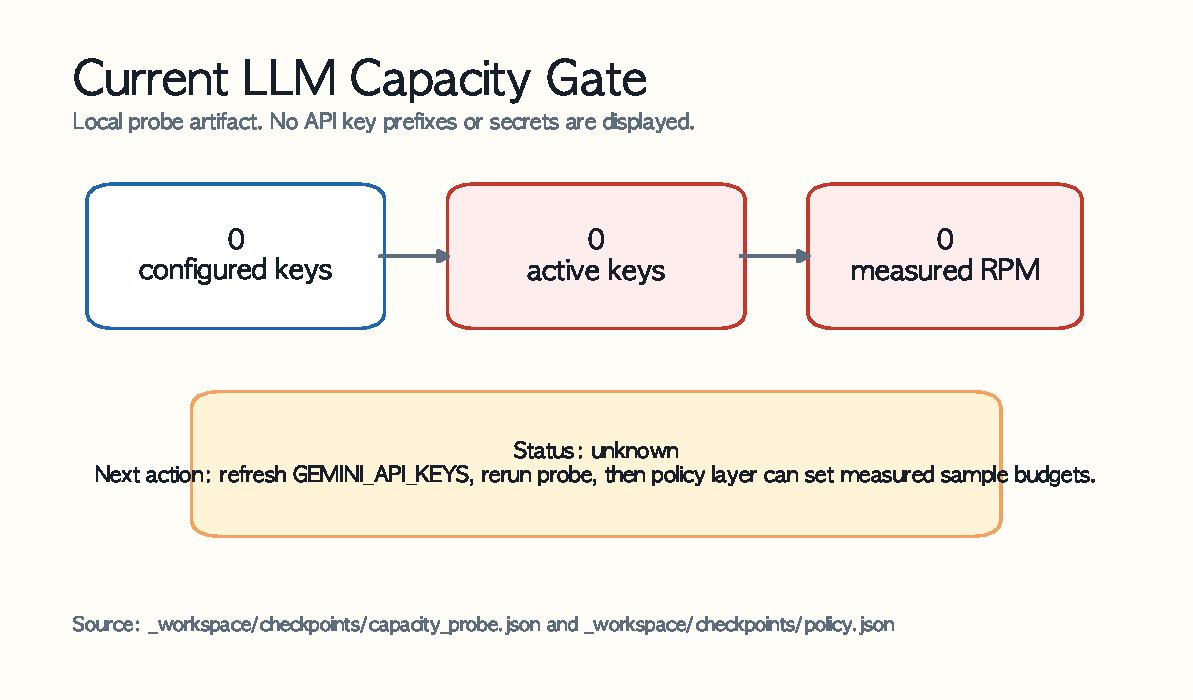
\includegraphics[width=0.84\linewidth]{assets/fig_capacity_gate.pdf}
\caption{Capacity-gating 요약. 초기 synthetic 48 RPM envelope는 full prompt workload를 과대평가했으며, 현재 planning에는 thinking을 끈 realistic payload probe의 46 RPM 결과를 사용한다.}
\label{fig:capacity-gate}
\end{figure}

\begin{table}[h]
\centering
\caption{지역별 capacity 기반 설정. probe 이후 \texttt{\_workspace/checkpoints/policy.json}에서 채운다.}
\label{tab:capacity}
\small
% TODO: fill from _workspace/checkpoints/policy.json
\begin{tabular}{llrrrl}
\toprule
지역 & 유형 & $n$ 페르소나 & $T$ 시점 & 동시성 & 기능 플래그 \\
\midrule
서울시장 & metropolitan\_mayor & TBD & TBD & TBD & TBD \\
광주시장 & metropolitan\_mayor & TBD & TBD & TBD & TBD \\
대구시장 & metropolitan\_mayor & TBD & TBD & TBD & TBD \\
부산 북구갑 & national\_assembly\_by\_election & TBD & TBD & TBD & TBD \\
대구 달서갑 & national\_assembly\_by\_election & TBD & TBD & TBD & TBD \\
\bottomrule
\end{tabular}
\end{table}

\subsection{KG Schema Reference}
\label{app:kg-schema}

표~\ref{tab:kg-ontology}의 ontology dataclass와 엣지 레이블은 \texttt{src/kg/ontology.py}에 정의된다. 이들은 \texttt{src/kg/builder.py}에 의해 \texttt{networkx.MultiDiGraph}로 컴파일된다. \texttt{src/kg/retriever.py}는 각 페르소나의 정보 상태 $I_{i,t}$를 만드는 GraphRAG subsampling을 구현하고, \texttt{src/kg/firewall.py}는 위에서 설명한 컷오프 $\tau(t)$를 강제하며, \texttt{src/kg/export\_d3.py}는 대시보드 KG viewer panel용 그래프를 직렬화한다. 표~\ref{tab:kg-ontology}와 함께 보고한 5개 지역 누적 그래프(212개 노드, 354개 엣지; 선거일 2026-06-03의 단일 공유 $Election$ 노드 \texttt{election\_2026\_local})는 모든 downstream 시뮬레이션이 사용하는 스냅샷이다. KG는 고정 입력이므로 이 수치는 sim-engineer run에 의해 변하지 않는다.

KG와 방화벽은 clean checkout에서 다음 명령으로 재현된다.
\begin{verbatim}
docker compose run --rm app python -m src.kg.builder
docker compose run --rm app python -m src.kg.firewall
docker compose run --rm app python -m src.kg.export_d3
\end{verbatim}
첫 번째 명령은 큐레이션된 시나리오 JSON 파일에서 \texttt{networkx.MultiDiGraph}를 다시 만들고, 두 번째 명령은 7개 방화벽 단위 테스트와 2026-04-25 5개 지역 회귀 테스트를 실행하며, 세 번째 명령은 대시보드 KG viewer panel이 소비하는 D3 친화 JSON을 덤프한다.

\subsection{방정식-코드 매핑과 기본 계수}
\label{app:eq-code}

제~\ref{sec:results}절의 정식화에 쓰인 각 효용 성분은 \texttt{src/sim/}의 Python callable로 구현된다. 표~\ref{tab:eq-code}는 현재 하네스가 제공하는 기본 계수와 함께 매핑을 제시한다. 모든 계수는 \texttt{ElectionEnv} 생성 시 읽는 환경변수 feature flag로 조정 가능하다.

\begin{table}[h]
\centering
\caption{스모크 실행에 사용된 기본 계수와 방정식-코드 매핑. 값은 보정 과정에서 정교화될 수 있다.}
\label{tab:eq-code}
\small
\begin{tabular}{p{0.18\textwidth}p{0.42\textwidth}p{0.32\textwidth}}
\toprule
항 & 구현(\texttt{src/sim/}) & 기본 계수 \\
\midrule
$U^{\text{base}}_{i,b,k}$ & \texttt{utility.py::baseline\_utility(persona, candidate)} & 거친 연령 $\times$ 학력 $\times$ 정당 prior; KOSIS에 미적합 \\
$\Delta U^{\text{media}}_{i,b,k}(I_{i,t})$ & \texttt{utility.py::media\_shock(events, candidate, t)} & \texttt{timestep $\le$ t} KG 사건의 부호 polarity 합 \\
$\Delta U^{\text{poll}}_{i,b,k}(t)$ & \texttt{poll\_consensus.py::bandwagon\_underdog} & $\eta^{\text{bw}}=0.3$, $\eta^{\text{ud}}=0.1$ \\
$\Delta U^{\text{gov}}_{i,b,k}(t)$ & \texttt{utility.py::second\_order(gov\_approval, party, position)} & 여당 multiplier $+0.5$, 야당 $-0.3$ \\
$\varepsilon_{i,b,k}(t)$ & LLM sampling으로 암묵 실현 & temperature $T = 1.0$(Gemini 3 family requires $T \ge 1.0$) \\
$\hat p_{b,k}(t)$ & \texttt{poll\_consensus.py::consensus(raw\_polls)} & 표본 크기 지수 $\alpha = 0.5$, 최신성 $\lambda = 0.05$ \\
\bottomrule
\end{tabular}
\end{table}

통합 여론조사 집계기는 다음과 같은 de-biased weighted mean을 구현한다.
\begin{equation}
\hat p_{b,k}(t) = \frac{\sum_{j \in \mathcal{J}(t)} w_j \big(y_{j,b,k}(t) - \delta_{\text{house}(j),b,k} - \delta_{\text{mode}(j),b,k}\big)}{\sum_{j \in \mathcal{J}(t)} w_j}, \qquad w_j = n_j^{\alpha} \cdot \exp(-\lambda \Delta t_j) \cdot q_j,
\end{equation}
여기서 $n_j$는 여론조사 표본 수, $\Delta t_j$는 현장조사 종료 후 경과 일수, $q_j$는 조사기관별 품질 점수다. 결과 객체는 추가로 \texttt{meta.voter\_stats}(calls, parse failures, abstentions)와 지역별 runtime 통계(\texttt{cache\_hit\_rate}, \texttt{total\_calls}, \texttt{mean\_latency\_ms}, \texttt{parse\_fail\_rate})를 가진다. 이들은 Phase 3 실행이 끝나면 calibration table을 채운다.

\subsection{Gemini 3 Flash 설정 메모}
\label{app:gemini3-config}

초기 v2 모형 \texttt{gemini/gemini-3-flash-preview}의 두 가지 비자명한 동작은 파이프라인 신뢰성에 실질적 영향을 주었고, 현재 기본값을 \texttt{gemini/gemini-3.1-flash-lite-preview}로 바꾼 이유이므로 기록한다.

\paragraph{Thinking token은 output budget에 포함된다.}
Gemini 3 family는 내부 ``thinking'' token을 방출하며, 이는 \texttt{max\_output\_tokens} 예산에 포함된다. 512 token 예산에서는 긴 persona-plus-context prompt에 대한 poll/ballot 응답의 약 97\%가 문자열 중간에서 잘려 ``Unterminated string'' JSON parse error로 나타났다. poll 및 ballot 호출 예산을 2048 token으로, virtual-interview 호출 예산을 3072 token으로 올리자 제~\ref{sec:qual-example}절의 서울 live run에서 이 실패가 제거되었다(parse-fail rate $0/15$). 다른 provider는 이 coupling을 보이지 않으므로 \texttt{LITELLM\_MODEL} 변경 시 적절한 예산을 다시 검토해야 한다.

\paragraph{최소 temperature 제약.}
Gemini 3에 대한 LiteLLM compatibility note에 따르면 sampling temperature가 $1.0$보다 낮으면 ``infinite loops or degraded reasoning''을 만들 수 있다. 따라서 ballot, poll-response, virtual-interview mode 전반에서 $T = 1.0$을 균일하게 설정한다(표~\ref{tab:eq-code}). 이는 안정적인 JSON 출력을 위한 대가로 다소 높은 특이 noise를 받아들이는 것이다. provider가 이 하한을 부과하지 않는 경우에는 mode별 temperature 차등화를 다시 도입한다.

\subsection{유권자 에이전트 Prompt Template}

유권자 에이전트는 페르소나 속성을 인코딩한 system prompt와 경선, 후보, KG 유래 맥락, instruction mode(\texttt{secret\_ballot}, \texttt{poll\_response}, \texttt{virtual\_interview})를 담은 user prompt를 받는다. 응답 schema는 JSON으로 제한된다.
\begin{verbatim}
{
  "vote": "<candidate_id|null>",
  "turnout": <bool>,
  "confidence": <float in [0,1]>,
  "reason": "<<=200 chars; omitted in secret_ballot>",
  "key_factors": ["<<=3 strings>"]
}
\end{verbatim}
\texttt{secret\_ballot} mode에서는 실제 투표의 비밀성을 모방하기 위해 \texttt{reason} 필드를 억제한다. \texttt{virtual\_interview} mode에서는 에이전트가 설명을 확장할 수 있으며, 그 transcript는 그림~\ref{fig:demographics-kg}의 정성 panel을 채운다.

\subsection{결정성 및 Seed}

층화 페르소나 표본 추출, KG 시간 slice, 통합 여론조사 smoothing은 단일 experiment seed에서 seed를 받는다. LLM 호출은 기본적으로 비결정적이다. 결정적 재실행은 \texttt{(persona\_id, scenario\_hash, timestep)}로 키가 정해지는 \texttt{llm\_cache.sqlite} 항목을 replay해 달성한다. 캐시 해시는 모형 이름, prompt, generation config를 포함하므로 이 중 어느 하나라도 바뀌면 해당 항목은 무효화된다.

\end{document}
